\documentclass[bsc,deptreport,twoside,parskip,singlespacing,notimes]{infthesis}

\usepackage{graphicx}
\usepackage{caption}
\usepackage{subcaption}
\usepackage{float}
\usepackage{listings}
\usepackage[colorlinks=true,allcolors=black]{hyperref}

\raggedbottom %lol

\title{Prophasis - An IT Infrastructure Monitoring Solution for Small and Medium-sized Enterprises}
\author{Cameron Gray}

\abstract{
This project focussed on systems for monitoring IT infrastructure, specifically
examining their suitability for the small and medium-sized enterprise (SME)
sector.


First it examined a selection of tools that are currently popular and evaluated
them based on several points that are important in an SME environment.  From
this research several key weaknesses with current tools and potential
improvements on these were identified. 


The main part of the project involved developing from the ground up, deploying
and testing  a new IT infrastructure monitoring system for use in SME
environments.  This has been named ``Prophasis''.


The design and structure of Prophasis has been set out in detail and how the
system was implemented, tested and deployed in real world environments was
explained.  Finally how the system behaved in these deployments was discussed
and evaluated.  Areas for further development were also identified.


In summary this project has demonstrated that existing systems for monitoring IT
infrastructure have some major drawbacks in terms of their suitability for use
in the SME environment.  Prophasis, which has been successfully developed and
deployed in a real world environment has improved on the shortcomings which were
identified with the existing systems and provides a solution for the SME sector.
}

\begin{document}
\maketitle
\section*{Acknowledgements}
I would like to thank my supervisor, William Waites for his help and support
throughout the project. I would also like to thank the members of The Tardis
Project and CompSoc IRC channels for their advice and suggestions for Prophasis.
Additionally I would like to thank my employer, Lynchpin Analytics Limited for
generously allowing me to test Prophasis on their IT infrastructure.  Finally,
I would like to thank my family for their help and support throughout my
university career.

\tableofcontents

\chapter{Introduction}
	In recent years, almost all businesses have been expanding their IT
	infrastructure to handle the modern demand for IT systems.  As these systems
	grow and become increasingly important for business operation it is crucial
	that they are sufficiently monitored to prevent faults and periods of downtime
	going unnoticed.  There is already a large range of tools for monitoring IT
	systems however they are  designed for use on massive scale networks managed by
	teams of specialised system administrators.  As a consequence they are
	complicated to set up and manage and multiple tools are often required to gain
	a suitable level of monitoring.


	Current tools generally either fall into the category of real time
	alerting (sending an alert when there is a problem) and time series
	monitoring (capturing data about the performance of systems and presenting
	graphs and statistics based on it). There is a large gap in the market for a
	tool that provide both of these in one package. Such a tool would reduce the
	time required to manage the system as it eliminates the need to set up and
	configure two completely separate tools.


	Current tools are also generally managed and configured through various
	configuration files split across different machines on the network. This means
	that in order to efficiently use these tools a configuration management system
	such as	Puppet or Ansible must be used. In an SME environment with limited IT
	resources, a completely self contained system is often preferable.

\chapter{Analysis of Existing Tools \& Suggested Improvements}
	This chapter investigates existing tools and then suggests improvements on
	these.  Firstly it will take a look at a selection of current tools which are
	widely used in industry.  It will then evaluate these to establish their 
	suitability for SME environments.  From here, several areas for improvement
	are identified.  Finally, suggestions are made as to how a new tool could be
	designed for use in SME environments.

\section{Analysis of Existing Tools}
\label{analysis-of-existing-tools}

This section will review current IT infrastructure monitoring systems and
evaluate them on several points as follows:
\begin{itemize}
	\item Support for time series monitoring and real time alerting
	\item How they can be configured to monitor custom metrics
	\item How are alert thresholds defined
	\item How configuration and custom code is delivered to nodes (if required)
	\item How the user configures the system
	\item How dependencies are handled
\end{itemize}
The tools being reviewed are Nagios which is generally seen as the ``industry
standard'' monitoring tool along with Icinga 2 which attempts to improve on
Nagios to provide a more modern solution. Munin and collectd were also
investigated as they focus on time series monitoring. Finally, OpenNMS is
investigated as this is a very comprehensive tool designed for large scale
networks.


\subsection{Time series monitoring and real time alerting}

	There is currently a lack of tools that support both
	time series monitoring as well as real time alerting in any reasonable capacity.
	Nagios and Icinga2 are mainly focused on real time alerting so do not have much
	in the way of support for time series monitoring.  Whilst additional plugins are
	available to perform basic graphing functionality, historical data
	cannot be used to make decisions when it comes to determining the overall
	health of a host. On the other hand, Munin is designed primarily as a tool for time
	series monitoring.  Therefore it has extensive functionality for graphing
	collected data but has no built in support for alerting about faults or working
	out the health of a system. Collectd, as it's name suggests is used to collect
	information about a system and can be used to transfer it across the network. It
	has no built in functionality for viewing or analysing the collected data,
	instead the data is stored in RRD files which can be processed with separate
	software such as RRDtool.  It it also possible to alert based on this RRD data,
	however this would require additional tooling or custom scripts which are
	non-trivial to configure and manage.  OpenNMS on the other hand supports both
	real time alerting as well as collection and visualisation of time series data.


	It was identified that that the majority of tools only support either real time
	alerting or time series monitoring.  This means that in order to gain both of
	these, two separate tools (e.g. Nagios and Munin) need to be installed,
	configured and maintained completely separately.  OpenNMS supports both and can
	be used perform both real time alerting and time series data
	collection/visualisation.

\subsection{Support for Custom Metrics}

	Nagios, Icinga 2 and Munin all operate in similar ways here through the use of
	simple scripts that can be written in any language.  Both Nagios and Icinga 2
	execute the shell script and use the exit code to determine the health of the
	output (e.g. Exit code 0 means ``OK'' and exit code 2 means ``CRITICAL'').
	\cite{nagios-custom}  They
	also read data from stdout which can contain more information about the status
	of the check.  Munin plugins are similar where the field name and a numerical
	value are written to stdout and then picked up by the plugin.  Plugins must
	also, when passed ``config'' as a command line argument, print out information
	such as the title of the graph. Collectd, in the same fashion as Munin, relies
	on a custom executable to write the collected data to stdout following a
	specific format.  OpenNMS primarily uses SNMP to collect data from remote
	hosts.  Custom SNMP modules can be built to monitor custom metrics. 
	Alternatively, OpenNMS can be configured to read XML or JSON data over HTTP
	from an existing web application.\cite{opennms-http}


	In this area, most current tools are all much the same in the sense that they
	execute scripts and parse the output. This can be quite fragile as a badly
	written script could fairly easily output data in the wrong format. Using exit
	codes to output the overall health of a check is also very restrictive as
	described in subsection \ref{classification-threshold-definitions}. Using SNMP
	such as OpenNMS gives a much more well defined interface for exposing data
	about a system however this requires extensive configuration on the host being
	monitored.  Using XML or JSON over HTTP with OpenNMS is another option however
	this would require a custom application to be developed to expose the API.

\subsection{Classification Threshold Definitions}
\label{classification-threshold-definitions}

	Both Nagios and Icinga2 classify the result of a check within the plugin itself
	by the plugin exiting with the appropriate exit code to define the
	result.\cite{icinga2-dependencies}\cite{nagios-dependencies} This
	means that the thresholds are also generally stored inside the plugin script.
	OpenNMS allows thresholds to be defined on the raw data however these are
	complex to configure and are essentially defined as either upper/lower limits
	or are based off of changes between two samples.\cite{opennms-thresholding}
	Because Munin and Collectd do
	not support real time alerting, there is no support for classifying data.


	This is a clear issue with current systems, with most of them classification is
	performed on remote machines meaning that the logic used for this along with
	any threshold values are located on every machine in the network making it
	difficult to update. This also means that classifications can only use the
	current data collected and can't easily use historical data when deciding on a
	classification.  OpenNMS is somewhat better in this respect as it performs
	classification on the monitoring server itself however thresholds are somewhat
	limited as instead of being able to use arbitrary logic (as can be done in
	the shell scripts used by Nagios and Icinga2), thresholds must be defined as
	upper/lower limits or be based off of changes between two data points.

\subsection{Code/Configuration Delivery to Nodes}

	Nagios, Icinga2, Collectd and Munin are configured through several different
	configuration files and scripts stored on the disks of the server running the
	monitoring as well as the hosts being monitored.  There is no built in
	functionality in any of these tools for distributing these files to their
	respective machines.  For this, separate configuration management tools such as
	Puppet or Ansible would need to be used.  OpenNMS does not have any component
	that runs on the remote hosts, instead relying on the SNMP protocol or JSON/XML
	to be served over HTTP from the remote hosts.  This requires extensive
	configuration to be performed on all remote hosts.  This configuration is
	completely separate from OpenNMS hence there is no way to manage the remote
	hosts from within OpenNMS.


	This is a clear area for improvement. In a SME environment with a
	limited number of machines, each with their own separate role, configuration
	management tools are often not deployed.  Deploying an existing tool
	in such an environment would be time consuming as configuration would need
	to be manually copied between hosts. In addition editing the configuration later on
	would be a manual process of logging into every machine and changing the
	configuration files manually. This risks creating discrepancies between
	hosts if one gets missed during an update or updated incorrectly.

\subsection{How the user configures the system}

	Nagios, Icinga2, Collectd and Munin are all configured entirely using
	configuration files stored on disk. OpenNMS configuration is stored in a
	variety of XML files on disk.  These can either be edited directly or through
	a web interface.  However, due to the complexity of the XML files, the web
	interface for configuration is very complex due to the vast number of options
	available.


	This is another area for improvement. While configuration files are suitable
	for tools targeted towards expert users, they require a rather in depth amount
	of knowledge about ow the system is configured.  When configuring the system,
	users will continuously need to reference large amounts of documentation. Using
	configuration files also provides no mechanism for input sanitisation allowing
	for broken configuration to be saved. OpenNMS's web interface does make
	configuration somewhat more accessible however it is somewhat complex and still
	requires reference to extensive documentation.
	
\subsection{How Dependencies are Handled}

	Nagios and Icinga 2 both handle dependencies as a rigid tree where hosts can
	be set as dependent on other hosts.\cite{icinga2-dependencies}
	\cite{nagios-dependencies}  There is however no support for redundancy
	where the availability of a service can be dependant on one of several hosts
	being available. This is increasingly common in modern environments which often
	include large amounts of redundancy and fail over capacity. Munin and Collectd
	have no dependency functionality due to its lack of real time alerting. OpenNMS
	does not have explicit functionality to define services which are dependent on
	multiple hosts, instead this can be
	accomplished by creating a "virtual node" which behaves the same as a regular
	node in the system. This can be then configured to run an external script which
	would check the health of all hosts in the service and return the health of the
	overall service.

	This is another area for improvement. In a modern environment it is
	important for a monitoring system to be able to understand redundancy. While
	OpenNMS could be configured to check the health of a service where
	redundancy/failover is in place, however is a very complex process requiring
	custom scripts to be written.\cite{opennms-redundancy}
	

\section{Improvements over Existing Tools}
	After looking into the weaknesses in existing offerings	Prophasis was designed.
	This tool was designed specifically for use in small and medium-sized enterprise
	(SME) environments. Such businesses may have a small IT team with limited
	resources or may not
	even have a dedicated IT team at all, instead relying on one or two employees
	in other roles who manage the business's IT systems in addition to their
	regular jobs. The system therefore needs to be quick to deploy and manage without
	a steep learning curve. In order to use the system efficiently there should
	be no requirement for additional tooling to be deployed across the company.

\subsection{Configuration Management}

	It should be possible to manage the configuration of the system from a single
	location.  Prophasis provides a responsive web interface where every
	aspect of the system's operation can be configured, Prophasis then handles
	distributing this configuration to all other machines in the system in the
	background. Custom code for plugins is handled in the same way; it is uploaded
	to the single management machine and is then automatically distributed to the
	appropriate remote machines when it is required.

\subsection{Time Series Monitoring \& Real Time Alerting}

	Prophasis provides both the ability to alert administrators in real time when a
	system fault is discovered and functionality to collect
	performance metrics over time. This data can be used to generate statistics about
	how the system has been performing.  This time series data can be used to both
	investigate the cause of a failure in post-mortem investigations and to predict
	future failures by looking at trends in the	collected data.

\subsection{Expandability}
	It is important that a monitoring tool can be expanded to support the
	monitoring of custom hardware and software.  Without this, Prophasis would be
	limited to monitoring the hardware and software that it was designed with.
	An example of this would be
	hardware RAID cards.  Getting the drive health from these types of devices can
	range from probing for SMART data all the way to communicating with the card
	over a serial port.  It is therefore crucial that Prophasis can be easily
	expanded to support custom functionality such as this. Prophasis therefore
	supports a system of custom ``plugins'' which can be written and uploaded to the
	monitoring server where they can then be configured to monitor machines. These
	plugins are designed to be self contained and to follow a well defined and
	documented structure.  This provides scope for a plugin ``marketplace'' therefore
	eliminating the need for every user to implement custom monitoring code for the
	systems they are using.

\section{What Prophasis is Aimed At}
	Prophasis is designed for monitoring the IT infrastructure of SMEs. This may
	consist of a network of several physical or virtual servers potentially split
	between branch offices and a central datacenter.  These environments usually
	contain tens of hosts rather than thousands.  Prophasis is designed to monitor
	networks such as this in a clear and intuitive way.  It is not designed for
	monitoring massive multinational networks with many internationally 
	distributed networks containing thousands of machines.

\chapter{Design}
	This chapter will explain the design of Prophasis and explain various different
	design decisions that were made.  First it will go into detail explaining
	the choice of different technologies used in Prophasis and will explain the
	reasoning behind these decisions.  Next it explains the terminology used within
	Prophasis to give a better idea how everything is structured. It will then
	explain the layout of the various components in the system and will go into
	detail about the purpose of each of these components and how they operate.
	It then goes into detail about the design decisions made for how Prophasis
	determines the overall health of a given host or service from the individual
	data points that it has collected.

\section{Technology Choice}
\paragraph*{Implementation Language}
	It was decided to use Python as the language of choice to implement Prophasis
	for many different reasons. It is available on practically all
	platforms and is usually bundled with most UNIX-like operating systems.  Python
	also abstracts a large amount of low level details away which both saves
	development time and prevents subtle, hard to find errors such as memory
	management issues.  Python also has a huge library of available packages along
	with a powerful and flexible package manager (pip) and package repository
	(PyPi).  This allows external libraries to be used to provide functionality
	instead of requiring everything to be implemented from scratch.  Development time
	is therefore saved and specialised, well tested and maintained code
	can be used to provide some of the functionality.  Pulling in packages from
	PyPi instead of bundling external libraries with Prophasis ensures that any
	external libraries are kept up to date and prevents any licensing issues that
	could arise from bundling code from other sources alongside the Prophasis
	source code.

\paragraph*{Communications Protocol}
	HTTP was chosen as a communication protocol for several reasons.  It is well
	supported and understood with a large variety of server and client libraries
	available.  Using a premade library has major benefits for development time,
	security and support. HTTPS provides suitable encryption and certificate
	validation technologies to secure the system. HTTP is also widely permitted
	through firewalls and can be routed through web/reverse proxies.  This means
	that Prophasis can be operated on most networks without causing problems with
	firewalling.  HTTP also includes methods for transferring simple data as well
	as large binary files which is required for sending plugins to remote agents.
	Originally an attempt was made to use SSH to implement communication between
	the core and the agent.  However, it was found that this introduced a huge
	amount of additional complexity on both the server and client, especially if
	the SSH server were to be embedded into the agent to keep it as a self
	contained application.  This additional complexity not only made maintenance
	and development harder, it also increased the risk of errors being introduced.
	SSH was also more difficult to route through restricted networks.  Another
	benefit of using HTTP is how many well documented HTTP libraries and servers
	there are available, this means that alternative agents can be implemented with
	ease versus SSH which would involve having to handle a custom wire protocol.

\section{Terminology}

	This section explains the terminology used throughout the system to give a
	better idea of how everything is structured.

\subsection{Hosts \& Host Groups}

	In Prophasis, a ``host'' refers to a single machine that is being monitored. To
	aid management and organisation, it is possible to organise hosts into ``Host
	Groups.''  These can be comprised of hosts or other groups and can be used in
	place of hosts when defining services and checks.  Hosts can be grouped in
	various ways such as their role (Web server, VM Host), hardware configuration
	(Hardware RAID, Contains GPU), location (Edinburgh Office, Datacenter) or any
	other way that makes sense given the specific implementation.

\subsection{Plugins}

	A ``plugin'' is a package that checks a single attribute of a system.  For
	example a plugin could check the CPU load of a given machine or be used to
	check the health of all the hard drives in a system.  Plugins are implemented
	as Python modules that implement a specific API, they can return both a ``value''
	(a numerical representation of the data they collected) and/or a ``message'' (a
	string representation of the collected data).  Plugins are then packaged in a
	.tar.gz archive along with a manifest JSON file which contains information
	about the plugin for use when it is installed.


	Plugins are automatically distributed from the core to remote machines and when
	executed by the agent the value and message are returned to the core for
	classification and storage in the database.

\subsection{Checks}

	A ``check'' is a named set of hosts/host groups and a set of plugins to be
	executed on them.  When a check is executed, all of the plugins specified in
	the check will be executed across all of the hosts specified in the check.


	Checks allow logical grouping of various plugins.  For example you may have a
	check for ``Web server Resource Usage'' which will execute plugins to check the
	CPU load and memory across all hosts in the ``Web servers'' host group.

\subsection{Schedules}
\label{methodology-schedules}

	A schedule defines when one or more checks are to be executed.  Each schedule
	can contain multiple ``intervals'' which define when the check is run.  An
	interval has a start date/time and a time delta that defines how regularly it
	is to be implemented.

\subsection{Services}
\label{methodology-services}

	A service is defined in terms of ``dependencies'' and ``redundancy groups''. Each
	dependency represents a host that must be operational for the service to work.
	A redundancy group can contain multiple hosts where at least one must be
	operational for the service to work.


	As an example, there may be a ``Website'' service that has a dependency on the
	single router but has a redundancy group containing multiple web servers.
	In this case, if the router fails then the website will be marked as failed.
	If however one of the web servers fails but at least one other web server is
	still operational, the website service will only be marked as degraded.


	The use of services provides a clearer view of the impact of a given failure on
	the functionality of the network.  It also allows alerts to be set up so that
	they are only triggered when the service functionality is severely impacted and
	prevents alerts from being sent out for host failures that do not have a severe
	impact.

\subsection{Alerts}

	In Prophasis, alerts are set up to communicate with a specific person/group of
	people in a certain situation.  Alerts are defined in terms of to/from stage
	changes where an alert will be sent if the state of a host/service changes from
	one state to another (e.g. ``ok'' to ``critical'').  These can then be restricted
	to certain hosts, host groups, services, plugins and checks.


	The system supports ``alert modules'' - Python modules that are used to send
	alerts using various methods.  Examples of alert modules could be email, SMS or
	telephone call.


	Multiple alerts can be set up to handle different severities of issues.  For
	example, if a redundant service becomes degraded, a SMS or email message may be
	sufficient but if a service becomes critical it may be desirable to use a
	telephone call to gain quicker attention.

\subsection{Classification}
	A classification defines how serious or important the data from a plugin is,
	for example, the CPU load being slightly higher than normal would probably be
	classed as a minor issue whereas a system not responding to checks from
	Prophasis would be likely to be classed as a critical issue. Table
	\ref{table-classifications} lists all the different classifications ordered
	by severity.

%TODO Height of rows without vdots
\begin{table}[H]
	\centering
	\caption{Different classifications that can be given to data ordered by severity}
	\label{table-classifications}
    \begin{tabular}{|c|l|l|}
    \hline
    Severity     & Classification & Notes                                       \\ \hline
    Most severe  & Critical       & ~                                           \\
    \vdots       & Major          & ~                                           \\
    \vdots       & Minor          & ~                                           \\
    \vdots       & Degraded       & Only applies to services                    \\
    \vdots       & Unknown        & ~                                           \\
    \vdots       & OK             & ~                                           \\
    Least severe & No data        & Plugin has never been executed on this host \\ \hline
    \end{tabular}
\end{table}

\section{System Structure}

	The system is split into three separate components; Agent, Core and Web. Web
	and Core share the same relational database allowing data to be shared
	between them.  Figure \ref{system_structure} shows the individual components of
	the system and how they all interact.

%TODO B/W?
\begin{figure}[H]
	\caption{Diagram showing the layout of the components of the system}
	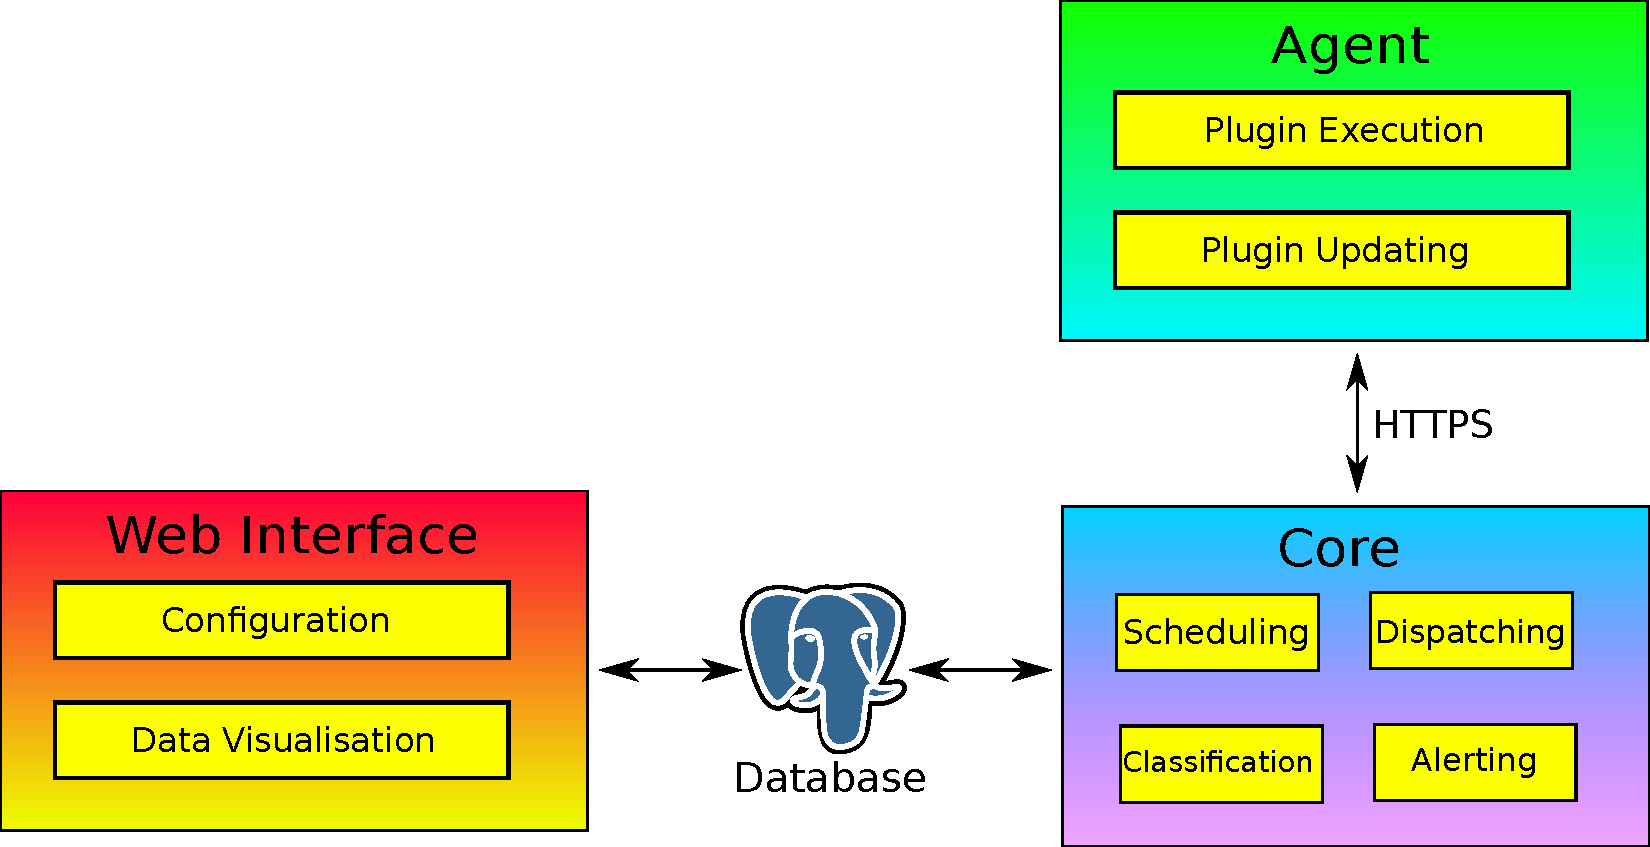
\includegraphics[scale=0.5]{assets/system_structure.pdf}
	\label{system_structure}
\end{figure}

\subsection{Agent}

	The agent runs on every machine that is being monitored and provides an API for
	communication with the monitoring server.  It listens on port 4048 (by default)
	and exposes an HTTPS API.  This API includes methods to check the version of a
	plugin currently installed on the agent, a method to push updated plugins to
	the agent and another method to execute a plugin and to retrieve the value and
	message produced by it.


	The agent's API is authenticated using a long, pre-shared key of which a salted
	hash is stored on the agent in a configuration file.  Being hashed prevents
	users who may have access to read the configuration file (possibly through
	misconfiguration) from getting the key to be able to communicate with the
	agent.

\subsection{Core}

	The core runs on the machine that is performing the monitoring, it has several
	different roles; scheduling, dispatching, classification and alerting.

\subsubsection{Scheduling}

	The core is responsible for looking at the schedules stored in the database and
	executing the appropriate checks on the correct hosts at the correct time.
	There is a configuration value for ``maximum lateness'' that defines how late
	after its defined time slot a check can be executed.  The core repeatedly
	checks the database looking at the intervals for each schedule along with the
	time at which a given schedule was last executed.  If it decides that a
	schedule is due to be executed it passes this onto the dispatcher.


	Figure \ref{scheduler_flowchart} describes how the scheduler operates.  Each
	schedule has a \linebreak\texttt{start\_timestamp} which is defined by the user
	when the schedule is created, an \texttt{interval} which is how often the
	schedule executes and a value for \texttt{execute\_next} which is the timestamp
	that the schedule is next to be executed.  When the scheduler starts up it
	first gets all schedules that do not have an \texttt{execute\_next} value -
	These are schedules that have never run.  It then calls
	\texttt{walk\_execute\_next} which is a simple algorithm that ``fast forwards''
	the \texttt{execute\_next} value until it reaches a timestamp that is in the
	future.  It then retrieves any schedules that are due to be executed
	(\texttt{execute\_next} is in the past) and executes them, it then calls
	\texttt{walk\_execute\_next} on each of these to set the \texttt{execute\_next}
	value to the time that the schedule should be run again.  The algorithm will
	then wait for 1 second before executing the process again.

\begin{figure}[H]
	\caption{Flowchart describing the operation of the scheduler}
	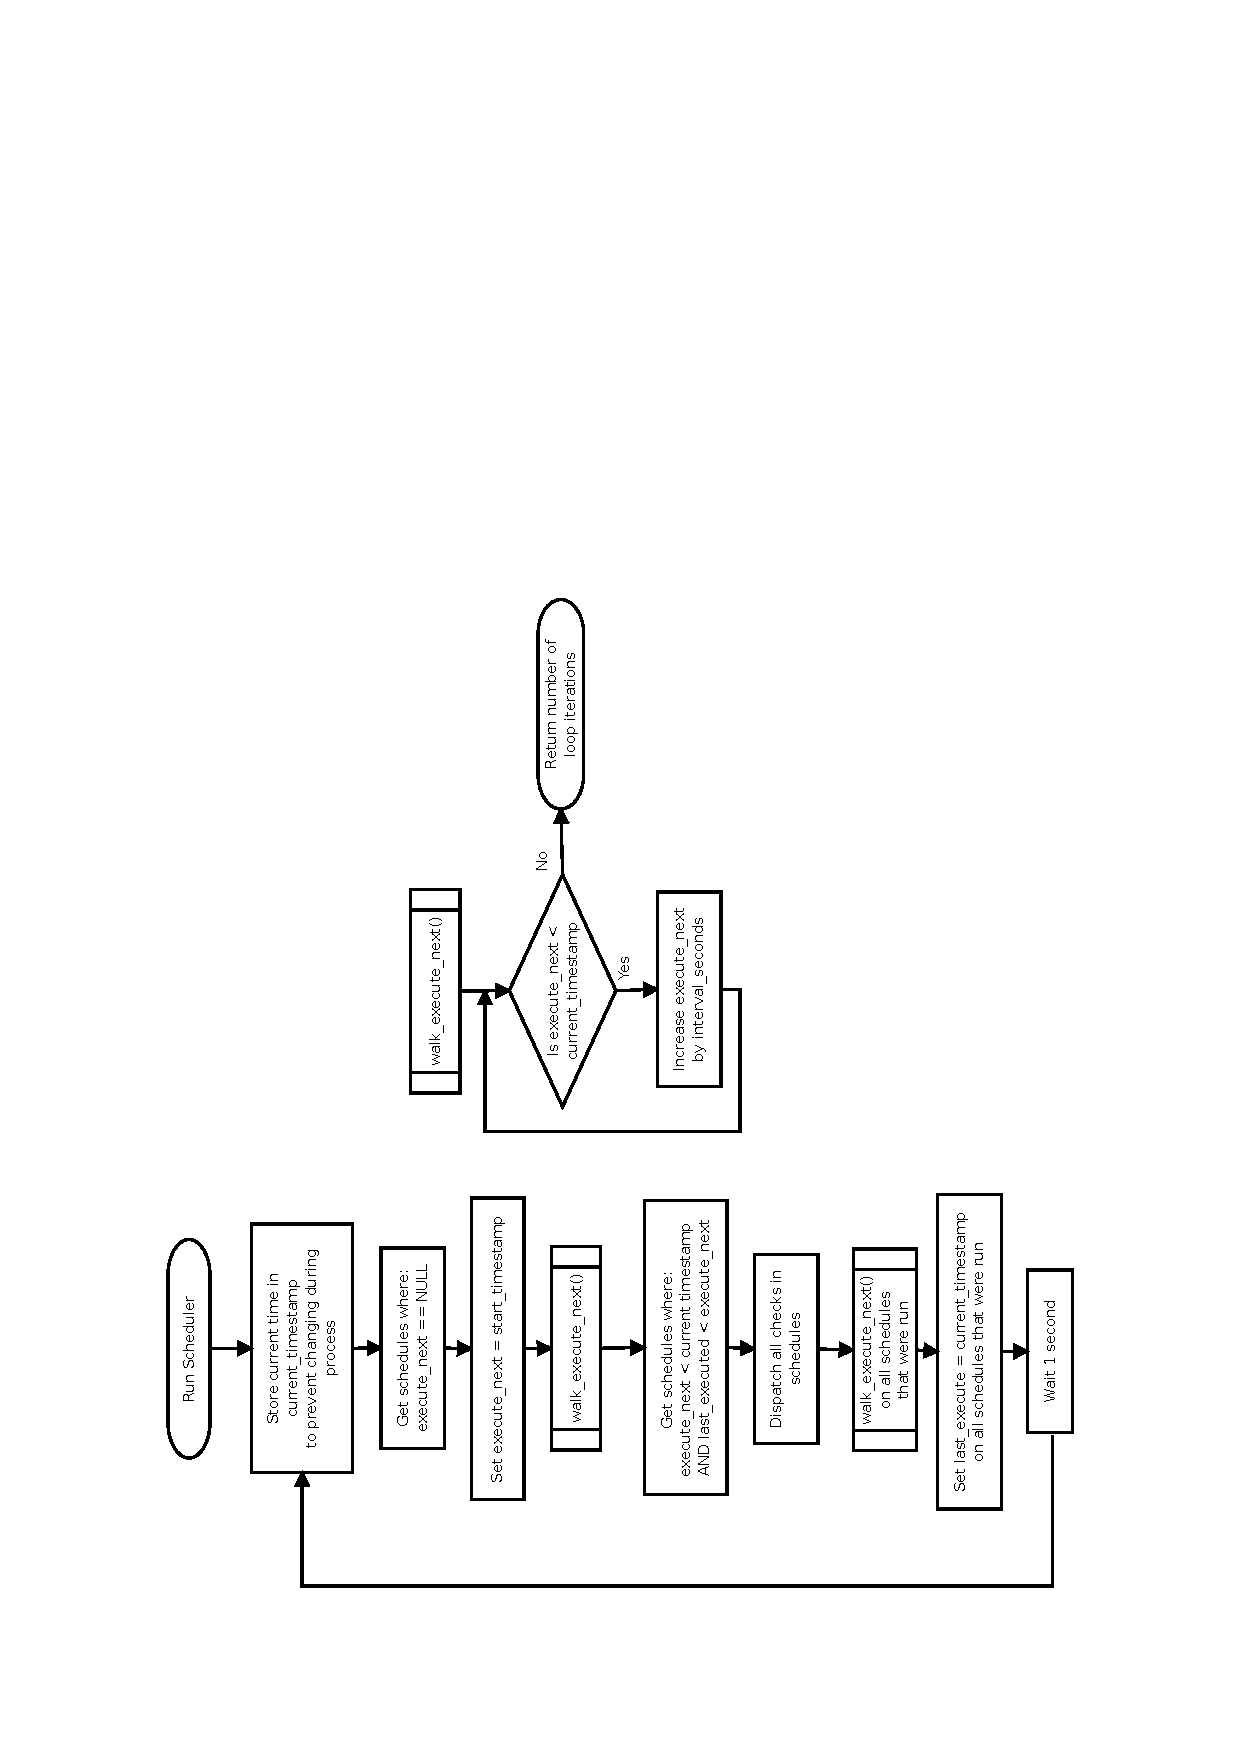
\includegraphics[scale=0.7, angle=-90]{assets/scheduler_flowchart.pdf}
	\label{scheduler_flowchart}
\end{figure}


\subsubsection{Dispatching}

	The dispatcher component of the core is responsible for issuing checks to
	agents when they are due to be run (as decided by the scheduler).  Checks may
	take some time to execute so executing these all in series would all be
	impractical. The solution for this was for the dispatcher to spawn a process
	for each agent that it is currently executing checks for.  Each process
	maintains a queue of plugins that are due to be executed and issues them to the
	agent in the order that they were dispatched.  This way only one plugin can be
	executing on a given agent at any moment in time.  This both prevents agents
	from becoming overwhelmed and means that plugin developers do not need to be
	concerned about other plugins interfering with their plugin.  Figure
	\ref{dispatcher_flowchart} shows the operation of the dispatcher.

\begin{figure}[H]
	\caption{Flowchart describing the operation of the dispatcher}
	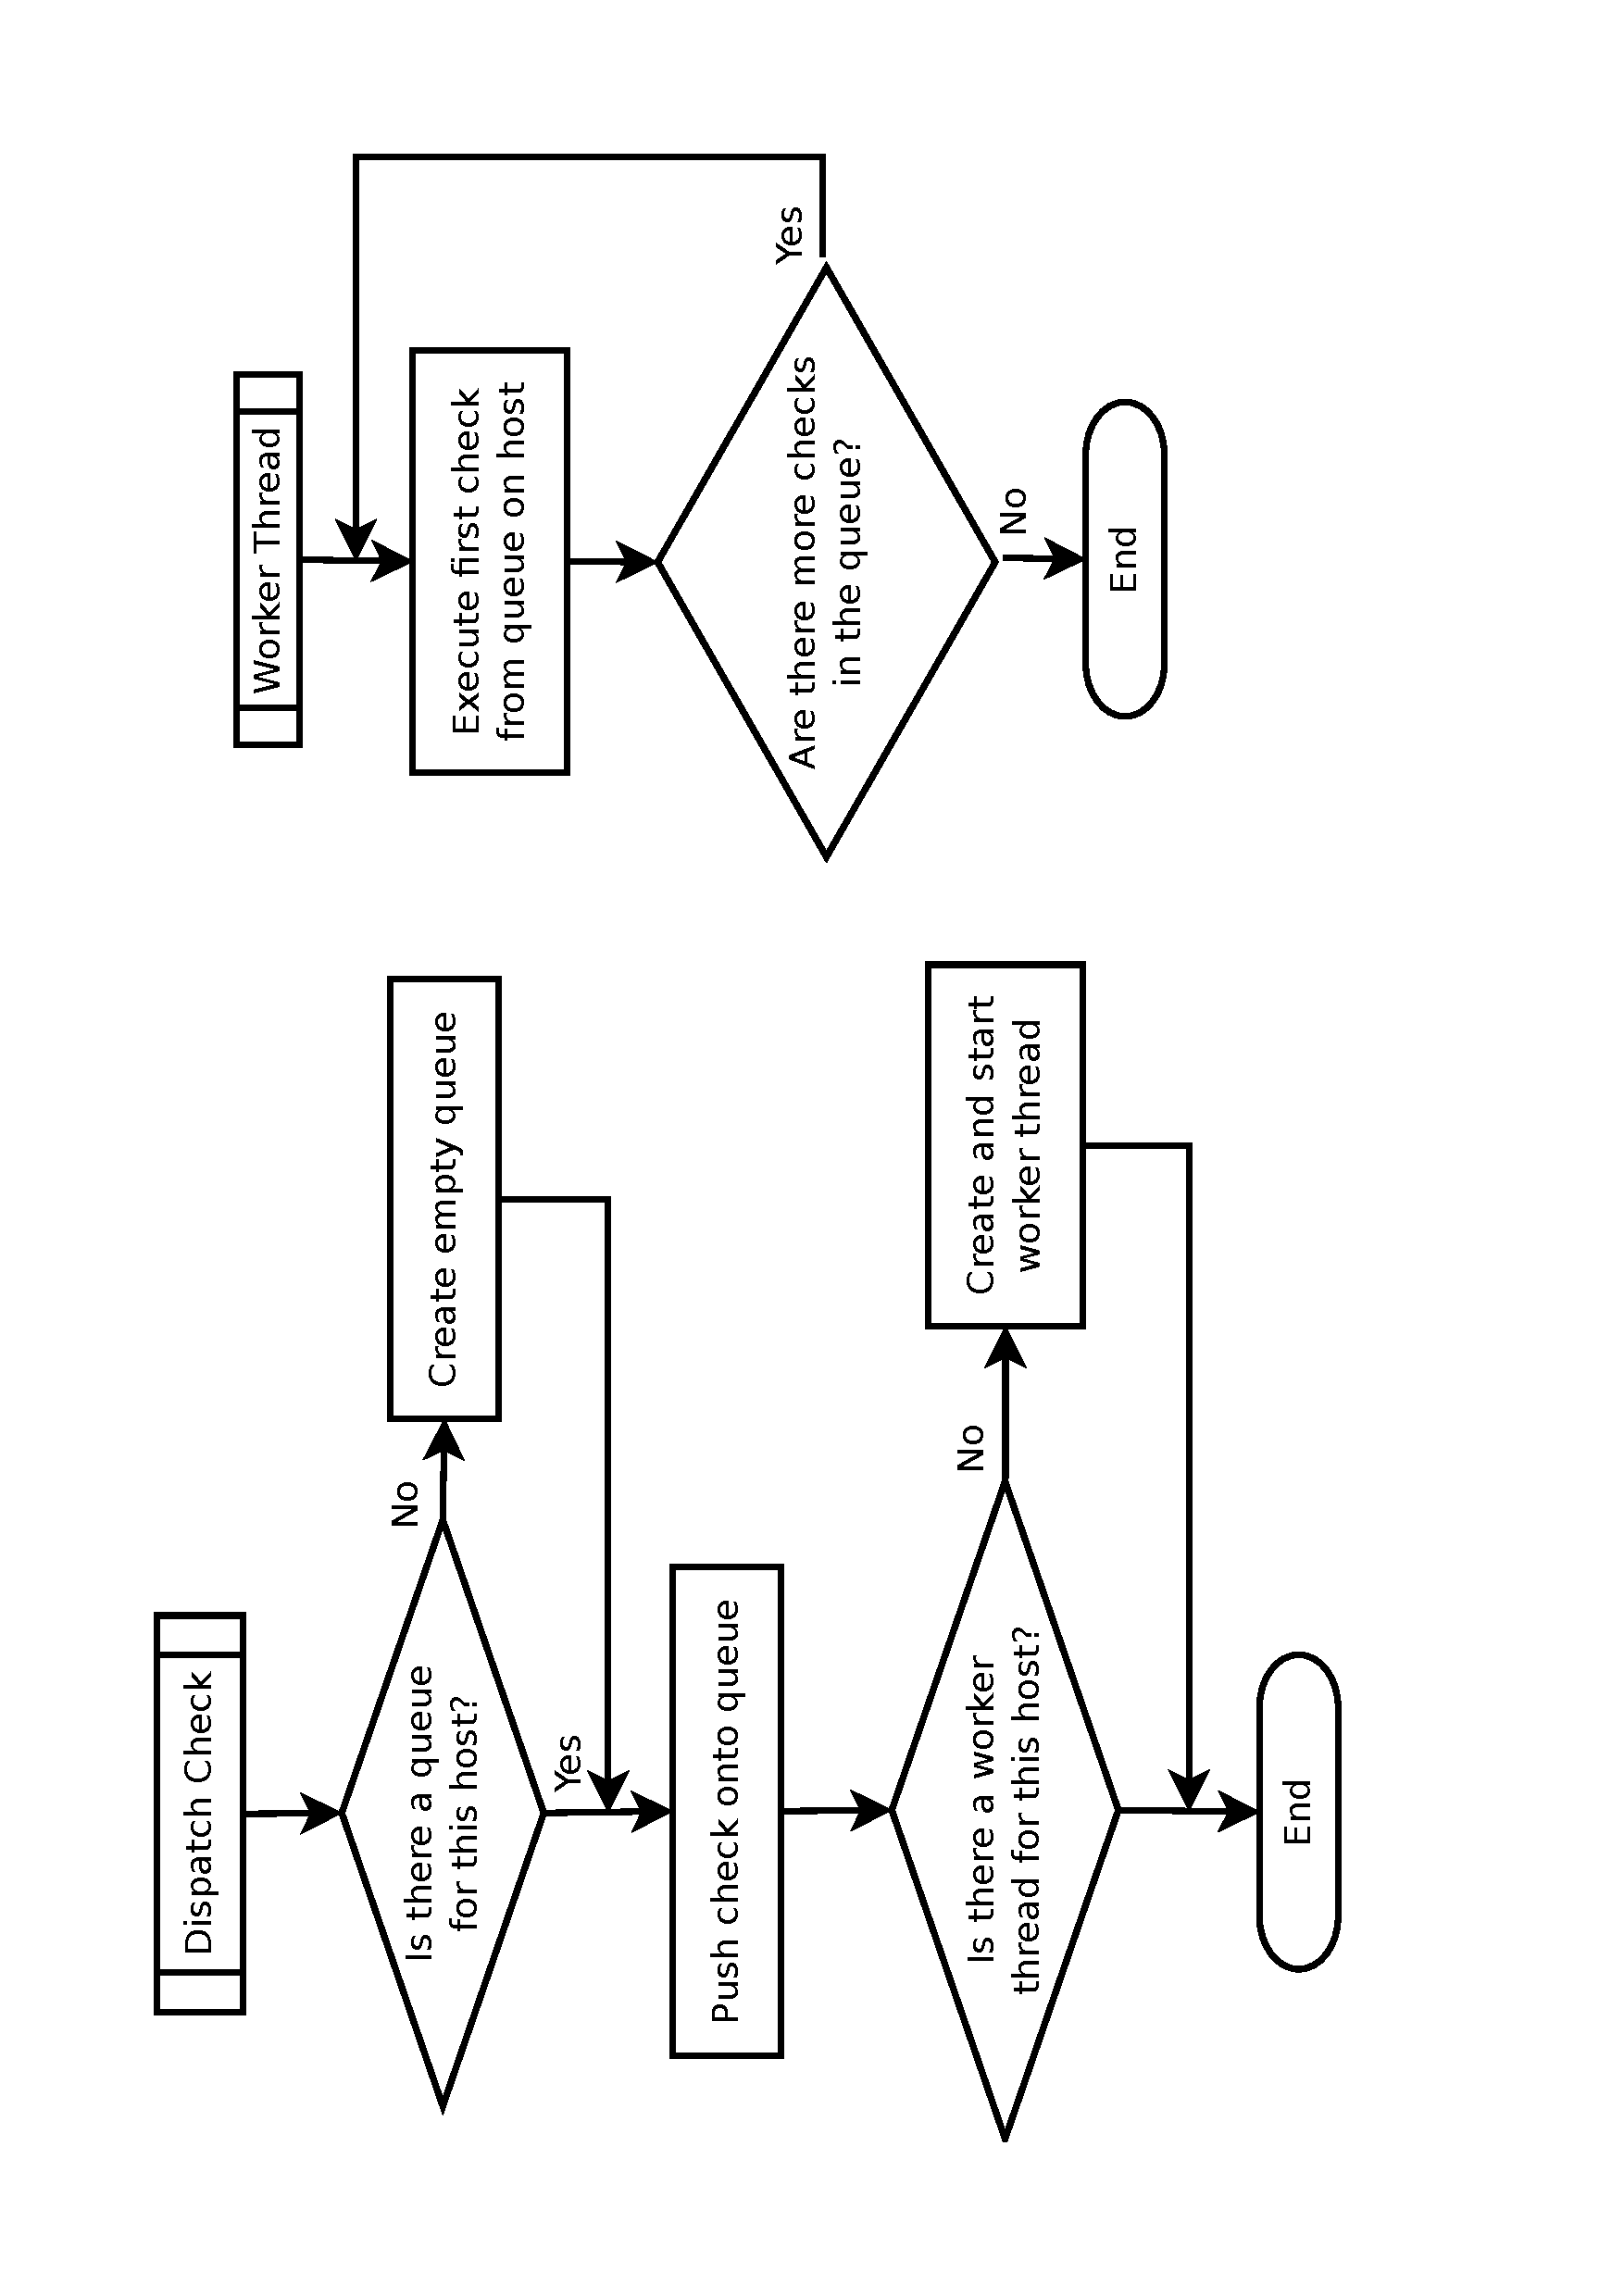
\includegraphics[scale=0.8, angle=-90]{assets/dispatcher_flowchart.pdf}
	\label{dispatcher_flowchart}
\end{figure}

\paragraph*{Communication Between Core and Agent}
	When a check is dispatched, the core and agent communicate to first of all
	establish if the agent already has the correct version of the plugin due to be
	executed installed. If it does not then an update will be sent to the agent.
	Once this is done the core will then request the agent to execute the plugin
	and the data will be returned for classification.  Figure
	\ref{core_agent_communication} describes the communication between the core and
	the agent.

\begin{figure}[H]
	\caption{Flowchart describing the communication between the core and the agent
		when a check is dispatched}
	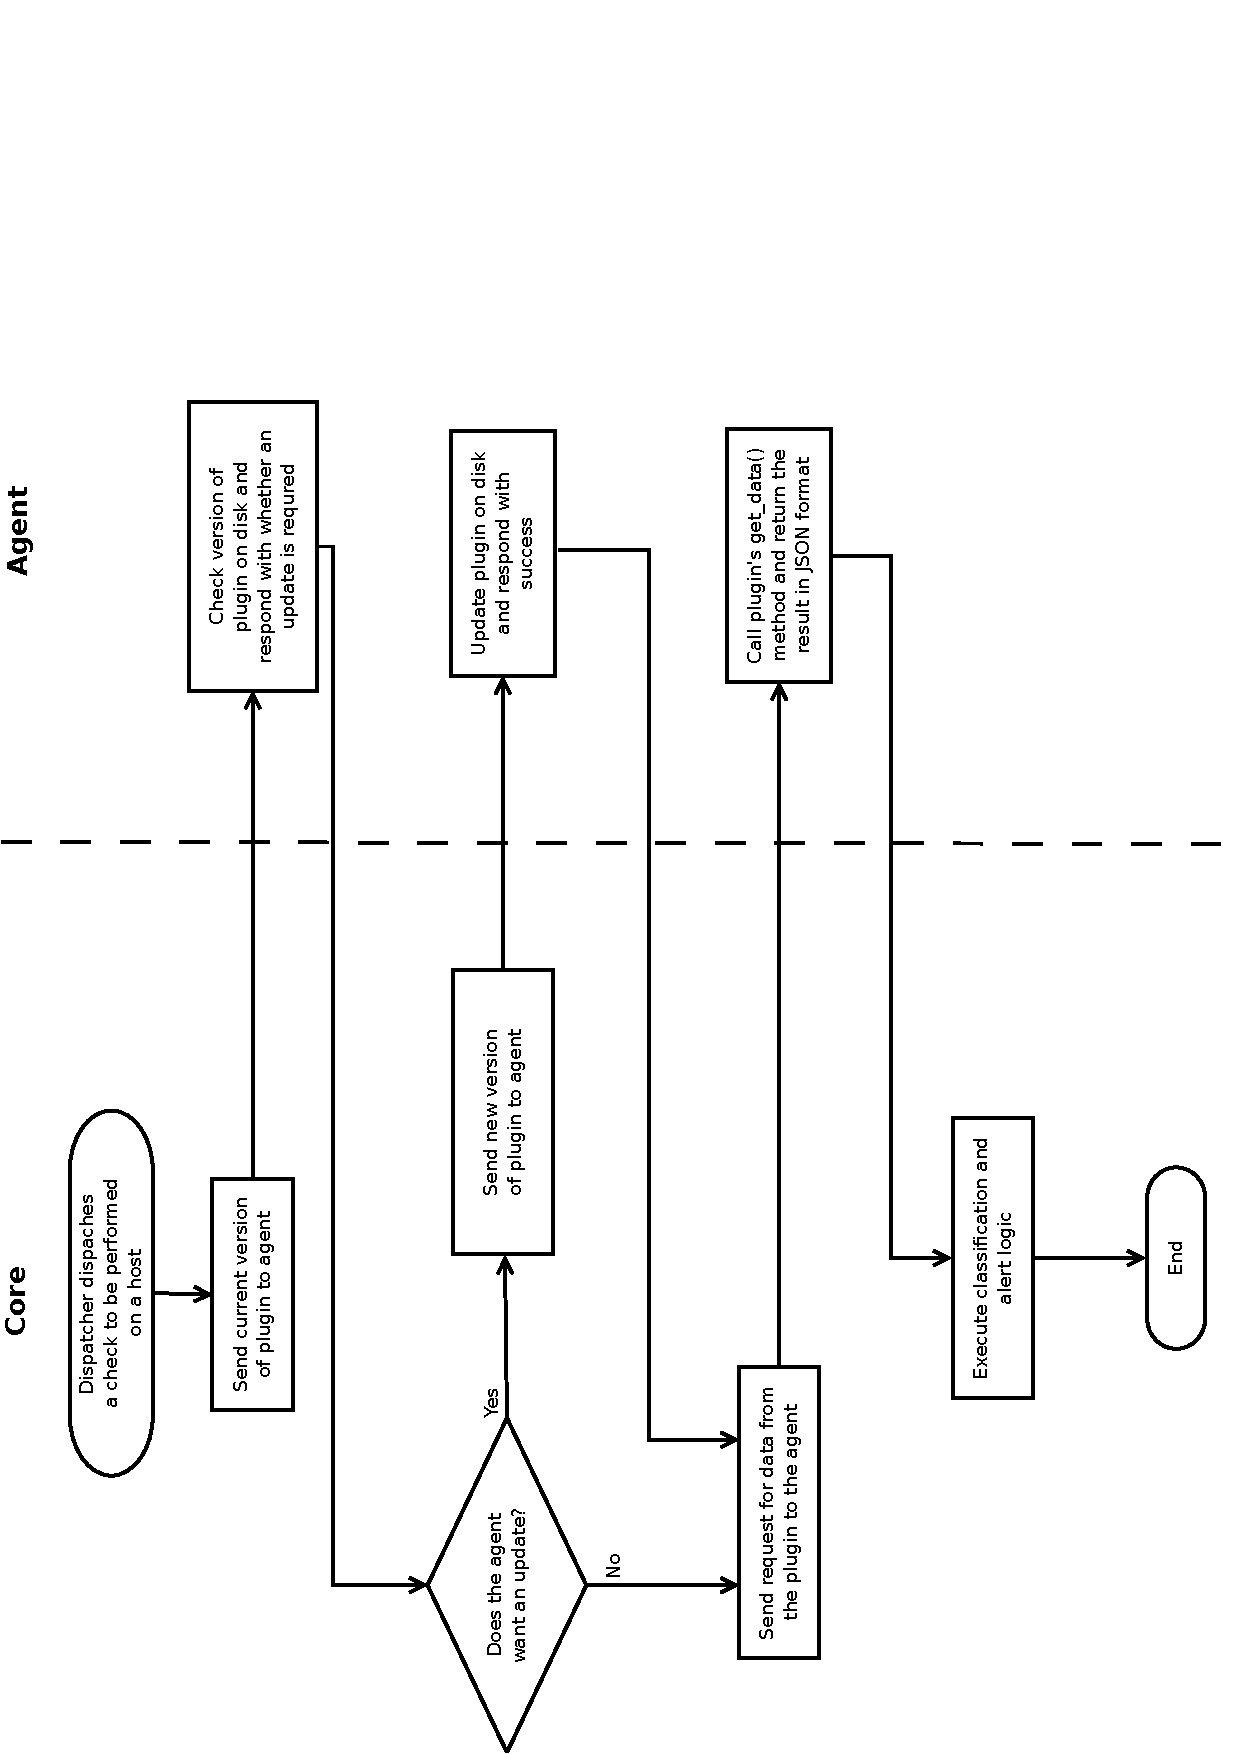
\includegraphics[scale=0.6, angle=-90]{assets/core_agent_communication.pdf}
	\label{core_agent_communication}
\end{figure}

\subsubsection{Classification}
\label{core-classification}

	When data is collected from an agent, it needs to be classified as ``ok'',
	``major'', ``minor'', ``critical'' or ``unknown''.  Classification is performed by Lua
	code that is stored alongside each plugin.  When the core finishes collecting a
	from an agent it will retrieve the classification code for the plugin and
	execute it in a sandboxed Lua runtime environment.  The result of the
	classification is then stored in the database.  The use of Lua code provides
	total flexibility. Classifications can be as simple as comparing values to a
	threshold or could go as far as looking at previous historical values and
	classifying based on a trend in the data. Plugins define how many previous
	historical values they want to classify on ($n$), the plugin's classifier code
	is then executed with two Lua tables, one containing the previous $n$ ``values''
	stored and the other containing the previous $n$ ``messages''.

\subsubsection{Alerting}

	Once the core has classified a piece of data, it now needs to work out
	whether it needs to send an alert or not.  To do this it looks at the previous
	state for the plugin and host along with the current state.  It then looks
	through the database for alerts that match that state transition and are
	applicable to the host/plugin combination.  If any alerts match it will call
	the alert module to send the alert out to inform the necessary people about the
	state change.

\subsection{Web Interface}

	Prophasis provides a web interface for both configuring the system and viewing
	collected data.  The interface is designed to be clear and easy to understand
	for users.  It is also built to be fully responsive so will work correctly on
	mobile device without any loss of functionality.  Designing it to be responsive
	was the aim from the outset as servers often fail when the administrator may
	not currently be in easy reach of a computer so will need to use a mobile
	device to investigate the issue.


	The web interface will connect to the same database as the core, and will
	update the configuration data stored in this database and will retrieve
	the data about hosts.


	The web interface provides dashboards for visualisation of data collected from
	plugins.  The collected data can then be displayed using graphs, tables, lists
	of messages or any other way that suits the type of data collected.

\section{User Interface}

	The nature of a monitoring system means that it will often need to be used from
	mobile devices when systems need to be checked on the move or out of hours. This
	requires that Prophasis's web interface must work correctly on both mobile devices
	and conventional desktops and laptops.  It was therefore decided to build a
	responsive web interface that will scale automatically based on the screen size
	of the device without any loss of functionality.


	In order to keep Prophasis as intuitive as possible, the user interface should
	contain clear explanations of different functionality as well as help text and
	detailed error messages.

\section{Determining the Overall Health of a Host or Service}

	In Prophasis, although the data returned by each plugin is classified individually,
	in order to display the collected data or to create alerts it is necessary to
	be able to decide on a general health classification for an entire machine or
	service based on the classifications for the individual plugins.

\paragraph*{Determining the health of a host}
	In order to determine the health of a host it is first necessary to establish what
	checks the host in question is part of. For this the database is queried to get
	a list of all checks the host is assigned to and then for each host group that
	the host is part of, all checks that the group is assigned to are fetched.  The next
	step is to iterate over the checks that have been found to build a de-duplicated list
	of all plugins that are being executed on the host in question. Then, for each
	plugin, the result of the most recent check of the plugin on the host is retrieved.
	Then, using the severity ordering in Table \ref{table-classifications}, the most
	severe classification from the plugins is chosen and this is used as the overall
	health of the host.

\paragraph*{Determining the health of a service}
	Determining the health of a service is somewhat less clear cut due to the use
	of dependencies and redundancy groups.  In Prophasis the health of all dependencies
	and redundancy groups in the service is obtained. The health of a redundancy group
	is taken as the least severe health out of all hosts in the group (unless the least
	severe is ``ok'' and there are non-``ok'' hosts in the group in
	which case the group is classified as degraded).  For example, a redundancy group
	containing a host with health ``minor'' and a host with health ``major'' would be
	classed as ``minor'' and a redundancy group with a host of health ``critical'' and
	a host of health ``ok'' would be classed as ``degraded''.  The overall
	health of each redundancy group is used along with the health of all dependencies
	(which is simply the health of the host that the dependency is for) and then
	the most severe of all of these is taken.  Severities are determined based on Table
	\ref{table-classifications}.


\chapter{Implementation}
	This chapter discusses the implementation of Prophasis and explains how all the
	individual components work.  It first explains the various technologies used to
	implement Prophasis going into detail about the libraries in use explaining
	the functionality that they provide.  It then explains the structure of each
	distinct part of the system, first explaining how plugins are structured before
	going on to explaining the database design.  It then discusses the core along
	with the functionality that this provides and then explains the operation of
	the agent. It finally explains the layout of the web interface and demonstrates
	various aspects of it's design.

\section{Technologies}

	The vast majority of the system is implemented in Python 3.  This allows for a
	large variety of modules to be used during development. Python is also widely
	available on UNIX systems and is easy to install on machines where it is not
	included.


	The Python ``Virtual Environment'' (Virtualenv) system is also extremely useful
	in this system.  It allows all dependencies to be kept totally separate from
	the rest of the system, this is particularly important for the agent as it
	ensures that the agent cannot interfere with the Python environment of the
	systems it is running on.

\subsection{Flask Web Framework}

	The agent and web interface are both built using the Flask web framework which
	handles routing URLs to the correct Python functions as well as handling
	request data and building the correct HTTP responses. The agent purely uses the
	routing and request/response functionality provided by Flask whereas the web
	interface also uses Flask's bundled templating engine, Jinja2, to render the
	HTML pages that are displayed to the user. The web interface also uses the
	Flask-Login package to provide login and user session management functionality.

\subsection{Tornado HTTP Server}

	While Flask does provide a built in web server, it is only designed for
	development	use.\cite{flask-deployment}  In order to provide a production
	suitable web server for the
	%TODO Did we use Tornado for the web interface too?
	agent.  Tornado uses the uWSGI interface provided by Flask.  Tornado was chosen
	as it can easily be integrated directly into the Flask application and
	therefore does not require any sort of external web server to be
	installed/configured on the system.

\subsection{SQLAlchemy ORM}

	All database functionality in Prophasis is handled through the SQLAlchemy ORM
	which abstracts the database into a set of Python classes (known as models).
	This not only reduces development time, it also reduces the likelihood of
	errors as all of the database queries are generated by the library rather than
	being handwritten.  The SQLAlchemy models file can also be shared between both
	the web interface and the core preventing duplication of database query logic.

\subsection{Lupa}

	Lupa provides an interface between the system's Lua runtime and Python.  It is
	used by Prophasis to execute the user provided Lua code that is used to
	classify the results of checks. A sandboxed Lua environment is configured to
	prevent this user provided code from performing undesired operations.
	Sandboxing is covered further in section \ref{classification_sandboxing}.

\subsection{PostgreSQL Database}

	Prophasis has been officially developed to support PostgreSQL databases,
	however through the use of an ORM it is possible to easily move to different
	database platforms such as MySQL or Oracle.  SQLAlchemy transparently handles
	the difference between different database platforms when generating its
	queries.

\subsection{Appdirs}

	Prophasis has been designed to support a variety of different operating
	systems.  Different platforms have different conventions for where an
	application should store configuration files and other application data.
	Appdirs is a Python library that works out the correct path for various types
	of files for the detected platform.  This means that files are stored in the
	correct directory no matter if Prophasis is installed on Linux, BSD, Windows
	or an other supported platform.

\subsection{AdminLTE \& Bootstrap}

	AdminLTE is an open source theme for building administration dashboards and
	control panels.  It is MIT licensed and is therefore compatible with the MIT
	licence Prophasis is built under.  AdminLTE is built on top of Twitter's
	Bootstrap framework which is well supported with a large range of plugins
	available.  AdminLTE and Bootstrap have extensive support for responsive user
	interfaces and therefore very little manual work needs to be done to make the
	user interface responsive to work well on both desktop and mobile devices.

\subsection{Handlebars.js}

	Handlebars.js is a very lightweight JavaScript templating engine.  It is used
	in the frontend of the web interface for rendering portions of the page that
	are generated after the page has loaded. In Prophasis alerts and items that are
	dynamically added to the DOM such as dependencies when editing services or
	intervals when editing schedules.  This means that any HTML logic can be
	totally separated from the JavaScript source code.  Unfortunately Handlebars
	templates are slightly different to Jinja2 ones.  For simply filling in
	placholders they are compatible with one another however, more advanced
	functionality such as conditionals and loops require slightly different syntax.
	Therefore care must be taken when rendering the same template with both Jinja2
	and handlebars.
	
\subsection{Stopit}

	Stopit is a Python library that provides an easy interface for setting timeouts
	on blocks of code or function calls.  This means that if the code inside the
	block takes longer than the timeout, it will be terminated and an exception
	will be thrown.  This is used to ensure that plugins do not take too long to
	execute.  Stopit can implement timeouts either by using multithreading or
	through the use of UNIX signals.  Prophasis uses the multithreading variant
 	since UNIX's \texttt{SIGALRM} is not supported under Microsoft Windows.

\section{Plugins}
	Plugins are bundles of code that are developed to monitor a specific aspect of
	a system, a plugin for example could be developed to monitor the CPU load of a
	system or to check the health of all RAID arrays on a given type of RAID
	controller.  Plugins are not bundled as part of the Prophasis distribution and
	are instead installed afterwards by uploading them through the web interface.
	

	Plugins are packaged as gziped TAR archives containing several different files.
	The contents of a plugin archive explained below.

\paragraph*{Manifest File}
	All plugins must contain a file to store information about the plugin called
 	\texttt{manifest.json}. Table \ref{table-manifest-contents} explains the
 	different attributes of the manifest file and if they are required or not.
 	The additional files described in the manifest file will be explained later in
 	this section.

\begin{table}[H]
	\centering
	\caption{The contents of a plugin's manifest file}
	\label{table-manifest-contents}
    \begin{tabular}{|l|l|c|}
    \hline
    \textbf{Key} & \textbf{Description} & \textbf{Required?} \\ \hline \hline
    name
    	& The name of the plugin
    	& Yes \\ \hline
    id
    	& \shortstack[l]{A unique identifier for the plugin,\\
    		e.g. com.example.plugin}
    	& Yes \\ \hline
    description
    	& A description for the plugin
    	& Yes \\ \hline
    version
    	& \shortstack[l]{Numerical plugin version, needs to be increased\\to ensure
    		agents are updated}
    	& Yes \\ \hline
    default\_n\_historical
    	& \shortstack[l]{Integer representing how many previous values \\
    		should be passed to classification logic. May\\be overridden from web interface.}
    	& Yes \\ \hline
    default\_classifier
    	& \shortstack[l]{File containing lua code to be used as the default\\
    		classifier.}
    	& Yes \\ \hline
    view
    	& Either the name of an built-in view or ``custom''
    	& Yes \\ \hline
    view\_source
    	& Name of the HTML file containing the view
    	& \shortstack[c]{If view\\is ``custom''} \\ \hline
    \end{tabular}
\end{table}

\paragraph*{Default Classifier}
	This is a Lua file containing the code that will be used by default to classify
	the data from the plugin.  This code will be loaded into the database on plugin
	installation and can be edited by users through the web interface.

\paragraph*{View Source Code}
	If a ``custom'' view is specified in the manifest file, an HTML file must be
	included to be used as a view for the data.  This HTML file is passed a list of
	collected data for the plugin for the date range specified for the report
	and is rendered using the Jinja2 templating engine.  Any HTML or JavaScript
	can be used to display the data as desired.

\paragraph*{Python Code}
	The plugin archive must be a Python module containing a class called
	\texttt{Plugin} which is a subclass of \texttt{PluginInterface}.  Therefore, an
	\texttt{\_\_init\_\_.py} file must be included.  There is no restriction to how
	the rest of the Python code in the plugin must be layed out however generally
	there will be a single Python source file containing the \texttt{Plugin} class
	which is exposed in \texttt{\_\_init\_\_.py}.

\subsection{Plugin Logic}
	The plugin is a Python module and can therefore contain any logic that it needs
	in order to be able to retrieve the appropriate data.  This may be as simple as
	using built in Python logic to get data such as CPU load, executing shell
	commands and parsing the result or reading system files.  However, the external
	interface for a plugin must follow a defined structure.  The structure of a
	plugin is shown in Figure \ref{plugin-uml}.

\begin{figure}[H]
	\centering
	\caption{UML diagram showing the structure of a plugin}
	\label{plugin-uml}
	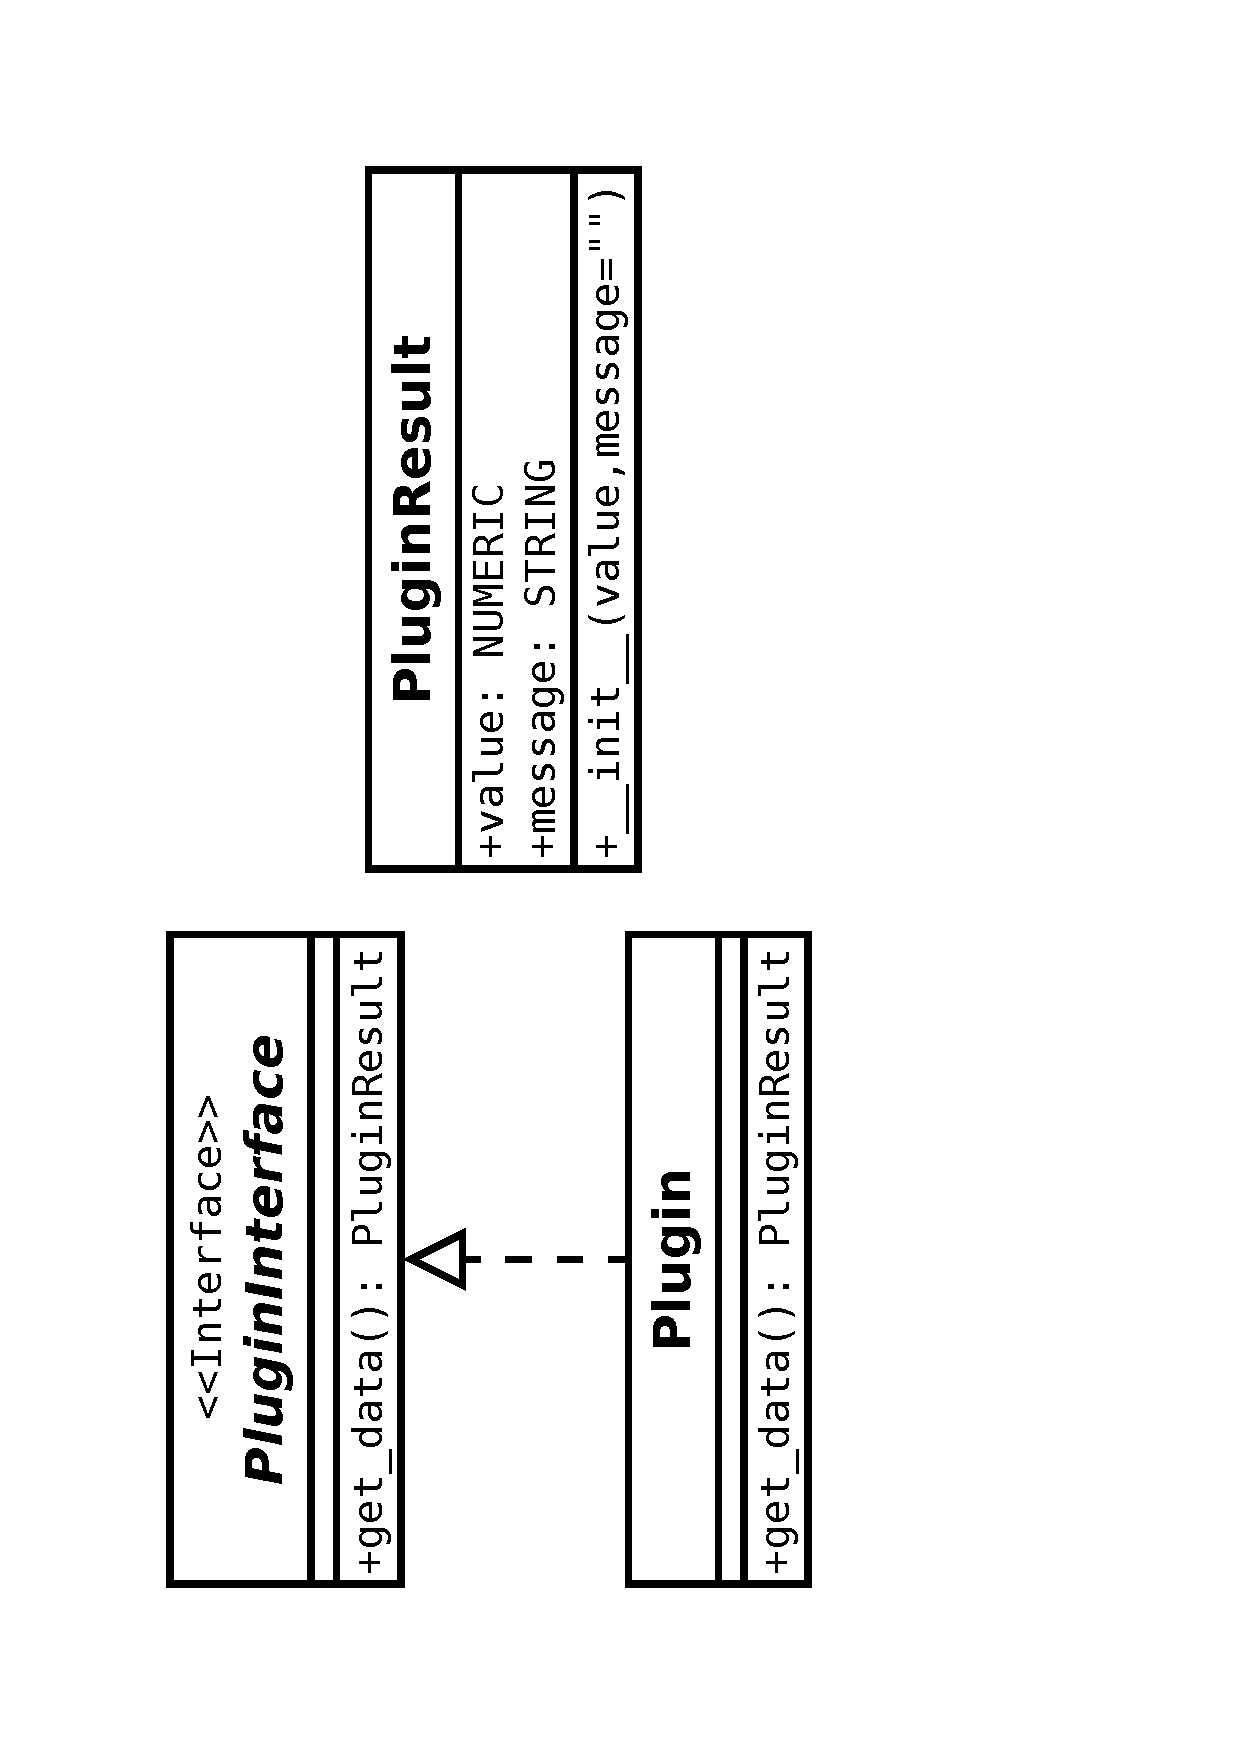
\includegraphics[scale=0.35,angle=-90]{assets/plugin-uml.pdf}
	\vspace{-5em}
\end{figure}


	All plugins must contain a class that extends from \texttt{PluginInterface}.
	This class must contain a \texttt{get\_data()} method which is called by the
	agent to get the data from the plugin.  The \texttt{get\_data()} method must
	return and instance of \texttt{PluginResult}.  The \texttt{PluginResult} object
	must contain a numerical value to represent the data collected by the plugin as
	well as a message which can contain more information about the data collected.
	The message defaults to being the empty string so does not need to be
	specified.


	The plugin's main class (the one containing the \texttt{get\_data()} method)
	must be exposed through \texttt{\_\_init\_\_.py} under the name \texttt{Plugin}.
	If the plugin's main class was called \texttt{CPULoad} in a module called
	\texttt{plugin.py} then it would be exposed using the line
	\texttt{from plugin import CPULoad as Plugin} in the \texttt{\_\_init\_\_.py}
	file.


	Structuring plugins in this way provides a large amount of flexibility.  The
	plugin can have any sort of internal implementation (it can even call out to
	shell scripts if desired) as long as the external interface follows the correct
	structure.  Forcing plugins to return data in the form of the
	\texttt{PluginResult} object forces them to return data in a sensible manner
	unlike existing tools which attempt to parse stdout of a shell script which is
	very fragile.
	
\subsection{PGP Signing}
	Since plugins are sent to agents over the network from the monitoring server 
	and then executed, This introduces a risk that if the monitoring server is
	compromised, malicious code can be sent to and executed on all hosts being
	monitored.  As a solution to this, it is possible to PGP sign plugins, a
	detached signature file can be uploaded along with the plugin archive file
	through the web interface, agents can then store public keys locally. If an
	agent is configured to enforce checking of signatures it will only allow
	plugins with valid signatures to be installed and executed.  Due to the
	additional complexity that this introduces, it is possible to disable this
	functionality although it is strongly recommended that it is used.  GNU
	Privacy Guard (GnuPG)\cite{gnupg} is used to verify signatures, this is
	available on most major operating systems.

\section{Database}

	The database is at the very center of Prophasis, it is used to store the
	configuration of the system along with data collected from agents, it is also
	the primary means of communication between the core and the web interface.
	Prophasis was designed to use the PostgreSQL DBMS and great care was taken to
	ensure that the database design was built to be efficient yet flexible enough
	to allow complex queries.


	The database was designed in a traditional manner using tables and relations
	between them in order to build an efficient and normalised design however it
	was implemented using the SQLAlchemy ORM which abstracts the database into a
	series of classes which saves time and reduces errors as queries do not need
	to be written manually.  The manual design was carefully implemented using
	extensive use of SQLAlchemy's \texttt{relationship()} function.  This allows
	relationships in the database to be traversed as easily as properties of an
	object.  For example, if you have an entity \texttt{h} of class \texttt{Host}
	and an entity \texttt{r} of class \texttt{PluginResult} then it is possible
	to both access a list of all plugin results attributed to the host with
	\texttt{h.check\_results} and to access, for example, the name of a host
	from the plugin result with \texttt{r.host.name}.  The ORM handles all the
	logic of building the queries to gather the correct data.  The ORM also makes
	it easy to edit data in the database, it is a simple case of retrieving the
	object, changing it's attributes and committing the session.  It is also
	transactional which means that changes can be staged up and then either
	committed or rolled back, this is ideal as it makes it easy to abort from
	changes to the database in the event of an error.  This also provides
	functionality to make multiple database operations atomic, this is important
	since there are multiple processes/threads writing to the same database.


	Figure \ref{database-diagram} shows a diagram that represents the structure
	of the entire database.  The colours have no significance and are simply used
	to illustrate which lines are crossing over and which are not.
	This diagram was built in a tool called Dia and stored
	in an XML file which could be kept on version control, this meant that
	throughout the development process the diagram could be easily maintained to
	match changes to the database, in fact, the diagram was always updated before
	the changes were applied to the actual SQLAlchemy models. Having this diagram
	available was extremely useful when developing parts of the logic that utilise
	the database as it makes the layout much clearer than simply reading the source
	code for the models file or by looking at the actual, running database
	instance.

\begin{figure}[H]
	\caption{Diagram representing the Prophasis Database Schema}
	\label{database-diagram}
	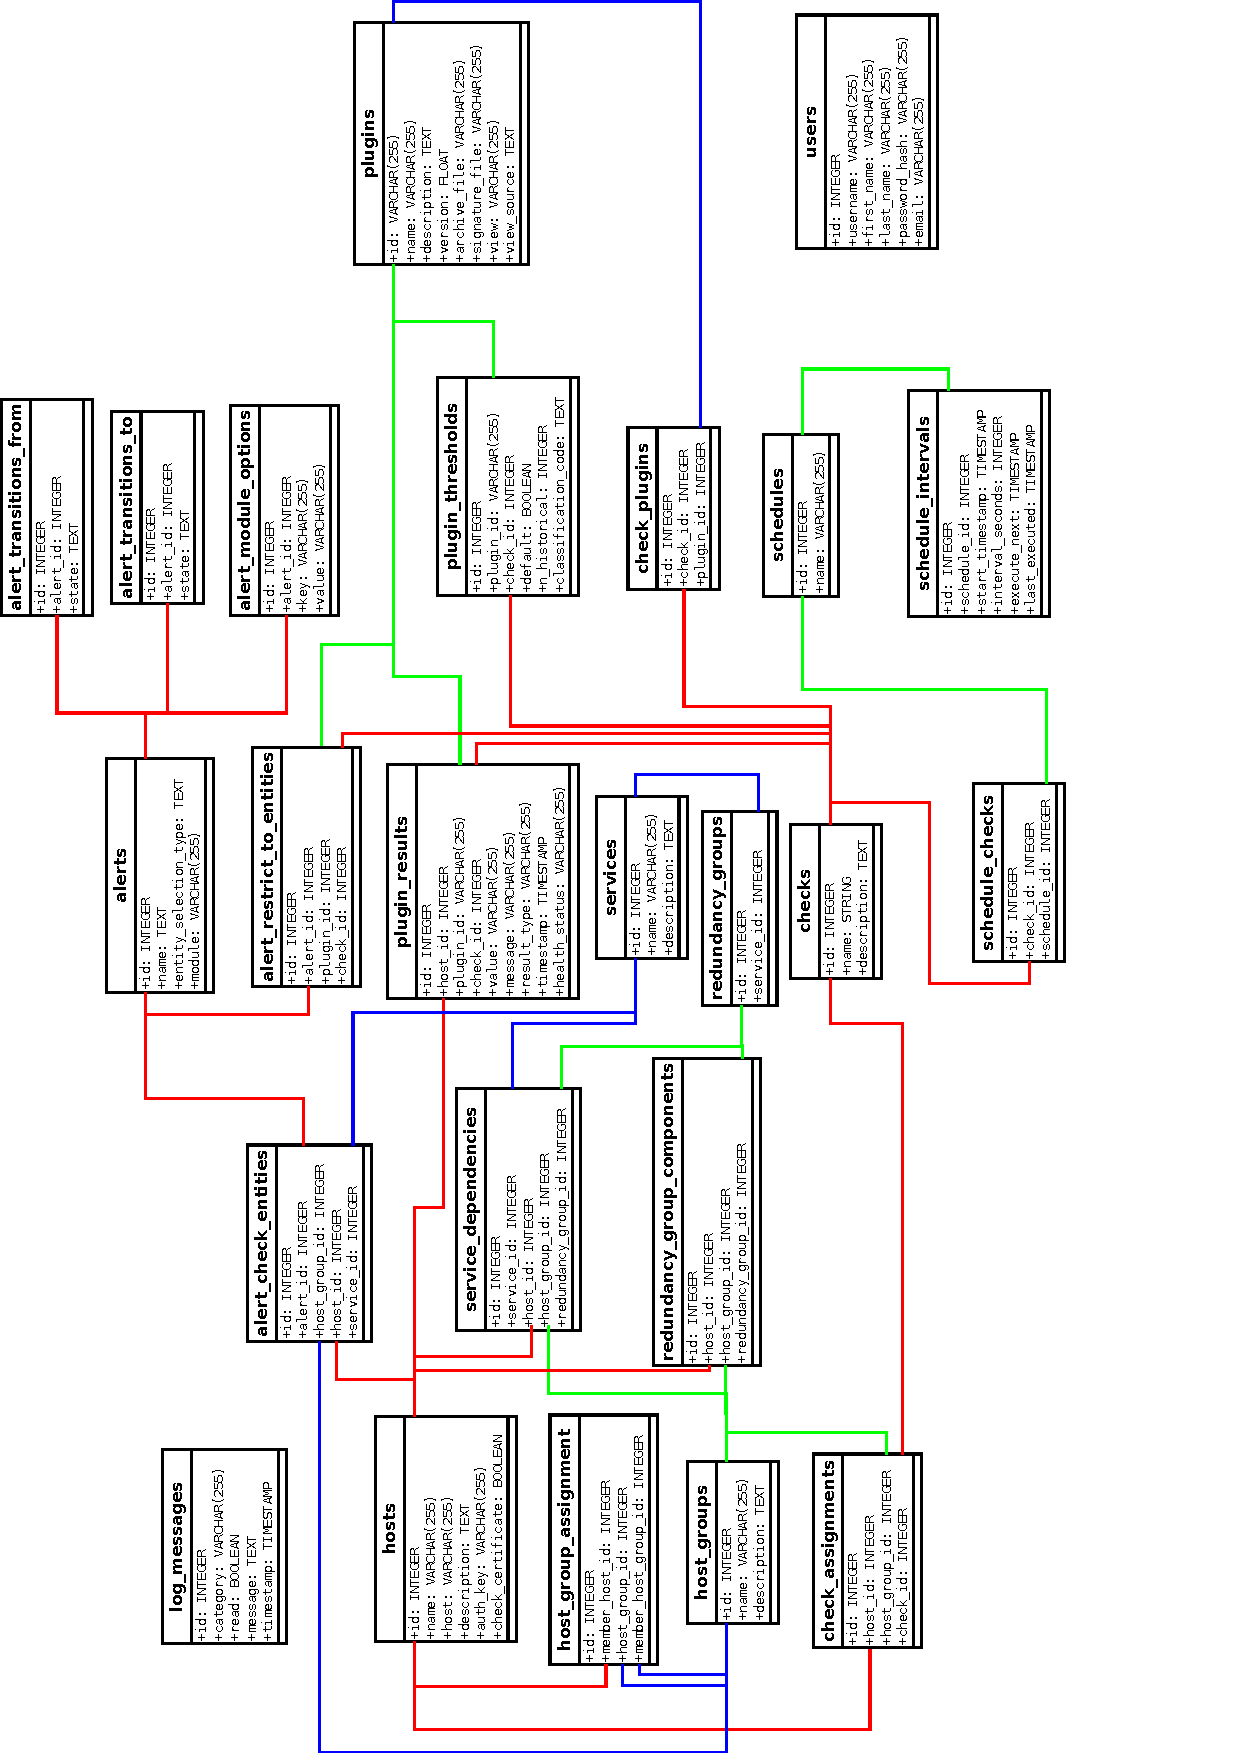
\includegraphics[scale=0.84]{assets/schema.pdf}
\end{figure}

\section{Common Module}

	Even though the core and web interface are completely separate processes, they
	still share some common logic: namely the database models, error logging and
	alert module handling.  It would be impractical to write this functionality
	twice, especially the database models as this is a huge piece of work.


	The best solution to this problem was to build a ``common'' python module known
	as \texttt{prophasis\_common}.  This contains the database models as well as
	error logging and alert module handling and is required by both the core and
	web interface.  When installing either of these the common module must be
	installed first.  Structuring the system this way prevents duplication of
	logic and ensures that there is no risk of there being any differences between
	the code in the core and the agent.

\section{Core}
\subsection{Dispatcher}

	The dispatcher is the system which sends off requests to the agent and waits
	for the responses back which are then classified and then stored in the
	database.  Due to the time it may take to execute some checks it would be
	impractical to execute them in series, therefore the dispatcher is
	multi-threaded.


	The Prophasis dispatcher uses Python's built in ``multiprocessing'' library. This
	provides various methods to manage processes as well as thread-safe data
	structures for communicating between them.  The dispatcher uses\linebreak
	\texttt{multi-threading.Process} to spawn worker processes and uses\linebreak
	\texttt{multiprocessing.Queue} to define thread safe queues for passing data
	into these worker processes.

\paragraph*{Fork vs Spawn}
	The multiprocessing library supports three different ways to start a
	process.\cite{multiprocessing-start-methods}
	By default on UNIX systems it uses \texttt{os.fork()} to fork the existing
	process. This is unsuitable in this situation as the process creates a copy of
	the already open database connection - this causes conflicts when the workers
	try to write to the database.  The solution to this is to tell the
	multiprocessing library to use the ``spawn'' context (the default on Windows)
	which will create a fresh Python interpreter process. This prevents open
	handles from being carried over into the child process. Using spawn is
	marginally slower than forking the process. In practice this not an issue however
	because processes are only spawned when schedules are called and these
	schedules are only called at most every second.

\subsection{Classification}

	When data is collected from the agent it needs to be ``classified'' to determine
	whether it is ``ok'', ``major'', ``critical''.etc.  Classification is done by Lua
	code that is bundled with the plugin and can also be modified by the user
	through the web interface.  The Lua classification code is stored in the
	database for ease of modification.  The ``Lupa'' Python library is used to
	integrate the Lua runtime into the Python code.

\subsubsection{Sandboxing}
\label{classification_sandboxing}

	Classification code is executed directly on the machine under the same user as
	the core.  Since this classification code can be changed through the Prophasis
	web interface it is critical that this code cannot perform malicious operations
	on the system.  In order to resolve this, a Lua sandbox is
	created.\cite{lupa-sandbox}  This is
	done by creating a Lua table with only specific, trusted functions such as
	\texttt{math} and \texttt{ipairs} added to it.  Lua's \texttt{setfenv} (set
	function environment) function is then called to ensure that all user provided
	code is executed inside this sandbox and can therefore not access more risky
	operating system functions such as file handling.

\subsubsection{Functions}

	In order to make developing classification code easier, several predefined
	functions are provided to handle common operations such as
	\texttt{arrayMax(array)} which will return the maximum value in an array and
	\texttt{arrayContains(array, value)} which returns a boolean defining whether
	the given value is in the array or not.  These functions are stored in a
	separate Lua file and are included before the user provided classification code
	before it is executed.

\subsubsection{Handling Errors}

	When dealing with user defined code there is always the potential for errors
	to occur when the classification code is executed.  In this situation the
	system will automatically fall back and classify the result as ``unknown''. The
	error will also be logged within Prophasis and can be easily viewed by the user
	in the web interface's ``System Logs'' area.

\section{Agent}

	The agent is implemented using the Flask web framework to expose a HTTPS API
	that the core communicates with.  Requests are sent to the agent using regular
	HTTP GET and POST requests with information passed using URL parameters or HTTP
	form data respectively.  Responses are formatted as JSON.  The Tornado HTTP
	server is used to handle incoming HTTP connections and communicates with Flask
	through using uWSGI.

\paragraph*{Authentication}
	In order to prevent unauthorised actions being performed on the agent, the core
	must authenticate with every request.  The agent stores a hash of a long
	authentication key in its configuration file. This key is generated during agent
	installation and is different for every agent. This ensures that if the key for
	one agent is obtained, an attacker cannot access every other agent on the
	network. Storing a hash means that if someone was able to read the agent
	configuration file they cannot obtain the authentication key which could have
	allowed them to execute code as the agent's user which may have higher
	privileges than their user. HTTP's basic access authentication is used which
	allows a username and password to be easily sent along with an HTTP request, in
	this situation the username is ``core'' and the password is the authentication
	key.  A Python decorator (\texttt{@requires\_auth}) is applied to functions
	that require authentication which will verify the authentication token and only
	allow the function to execute if the token is correct, otherwise it will
	respond with HTTP error 401 (Unauthorised). Using a decorator keeps
	authentication logic out of the body of the function which ensures that the
	user is authenticated before the function is even entered.  This prevents
	errors such as the authentication check being moved after some restricted
	functionality or accidentally being removed during changes to the function
	body.
	
\paragraph*{Plugin Execution}
	When a call is made to the Agent's \texttt{get-plugin-data} method, the agent
	will execute the plugin and return the data (value and message) returned by it.
	The agent uses \texttt{importlib.machinery.SourceFileLoader} to load the
	plugin's \texttt{\_\_init\_\_.py} file.  A new instance of the module's
	\texttt{Plugin} class is then instantiated and it's \texttt{get\_data()} method
	is called.  The data returned by this method is then returned to the core.
	It must be guaranteed that plugin execution will terminate in a timely manner
	as a plugin taking too long to execute will delay the execution of future
	plugins.  In order to ensure this, a timeout is set so that plugin execution 
	must complete within a predetermined amount of time, otherwise the execution
	will be terminated and an error will be logged by the core. The ``stopit''
	python library is used which uses threading to implement this.  Initially
	the ``timeout-decorator'' library was used however this uses the UNIX
	\texttt{SIGALRM} signal which is not supported by Microsoft Windows.

\section{Web Interface}

	The web interface is implemented using the Flask web framework.  The frontend
	is built using AdminLTE which in turn is based on Twitter's Bootstrap
	framework.  The web interface is built to be fully responsive so that it
	performs equally as well on both desktop and mobile devices.  The Jinja2
	templating engine is used to render the pages from HTML templates.  This allows
	certain pieces of template logic to be reused preventing code duplication and
	enforces a clear separation of logic between the processing and templating
	logic.

%TODO - Explain responsive design!
%TODO - Describe error logging to web interface.

\subsection{Configuration}

	All of the different configuration options are accessible through a clearly
	organised menu displayed on every page.  This allows the user to access all of
	the different configuration options from a single location.  This navigation
	bar can be seen in Figure \ref{settings-nav}.

\begin{figure}[H]
	\centering
	\caption{The ``settings'' navigation bar}
	\label{settings-nav}
	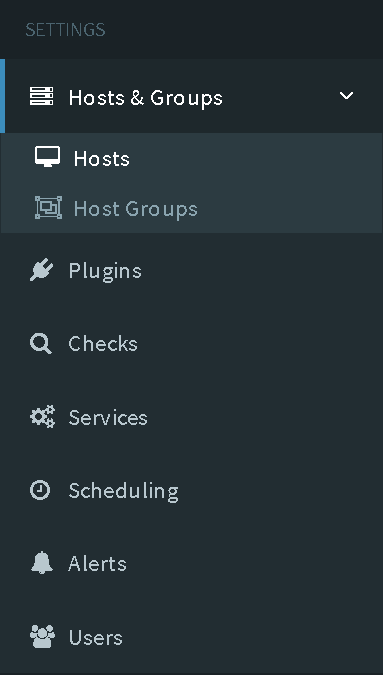
\includegraphics[scale=0.7]{assets/screenshots/settings-nav.pdf}
\end{figure}


	Clicking each of these links will take the user to the management area for
	that section allowing them to configure that part of the system.  The first
	page of any of these sections is an index page that lists all objects (e.g.
	plugins or alerts) in the section with options to manage each of them as well
	as providing a link to add new objects.  An example of the index page for
	alerts can be seen in Figure \ref{alerts-index}.  This page lists all alerts
	in the system and provides buttons to edit, delete and test them. There is
	also a button allowing the user to add new alerts to the system.

\begin{figure}[H]
	\caption{The alerts index page}
	\label{alerts-index}
	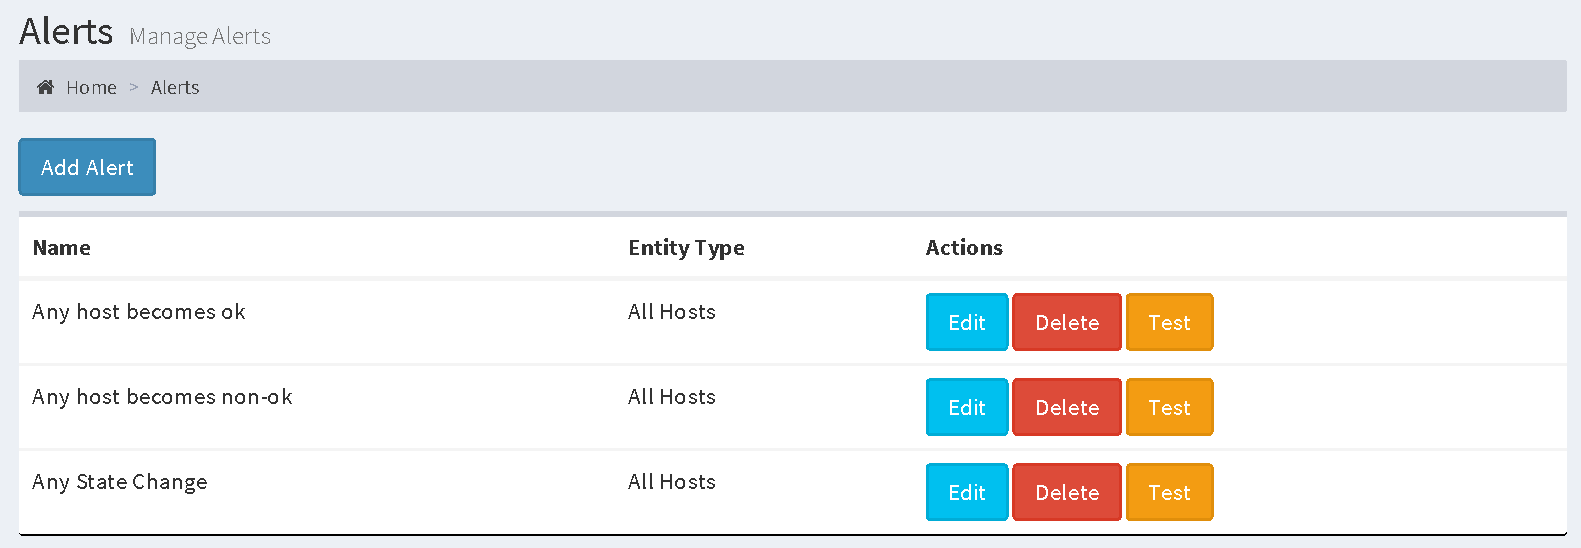
\includegraphics[scale=0.55]{assets/screenshots/alerts-index.pdf}
\end{figure}


	When the user chooses to add or edit an object a form is loaded.  The add and
	edit forms are both rendered using the exact same template files ensuring that
	both forms are consistent.  A \texttt{method} parameter is passed into these
	templates which is set to either ``add'' or ``edit''.  This is used to adjust the
	template.  Figure \ref{edit-check} shows the form for editing a check.

\begin{figure}[H]
	\caption{The Edit Check form}
	\label{edit-check}
	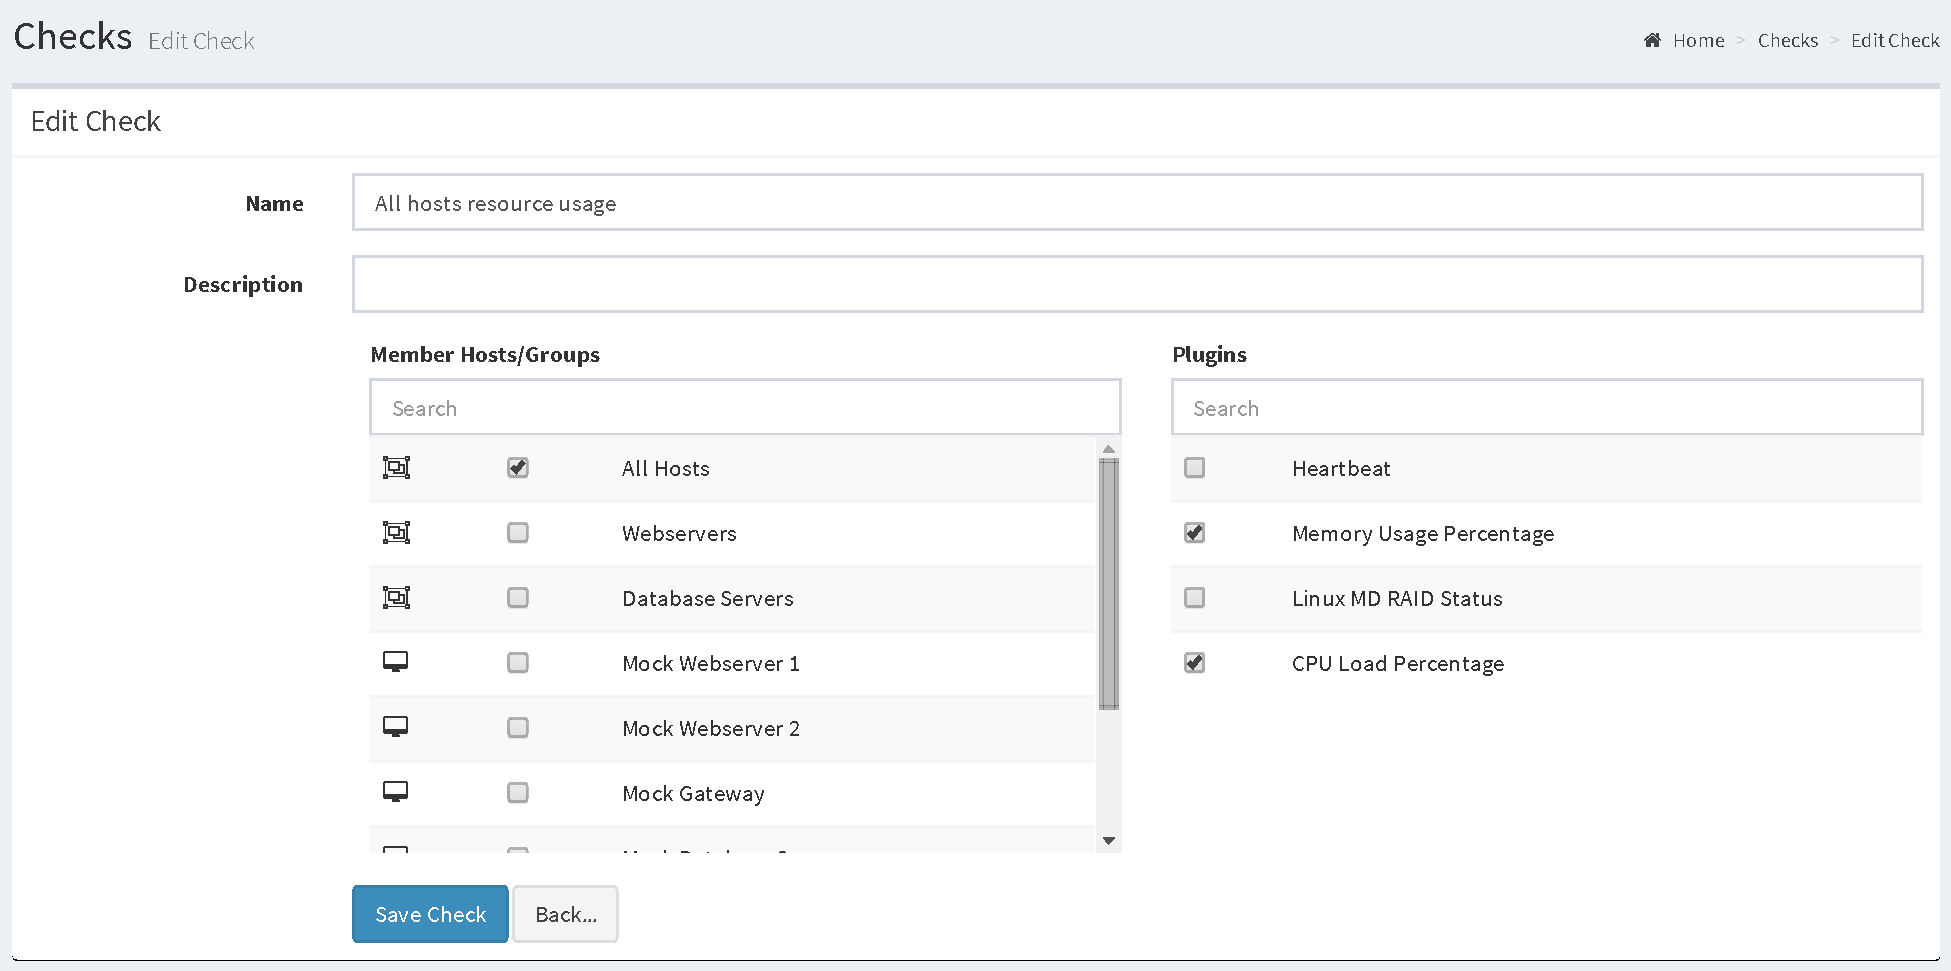
\includegraphics[scale=0.45]{assets/screenshots/edit-check.pdf}
\end{figure}


	This form has a pair of text boxes to specify a name and description for the
	check and then a pair of lists of checkboxes: the first lists hosts and host
	groups that the check will be executed on and the second lists plugins that
	will be executed on those hosts when the check is run.  The search boxes above
	each of these lists will filter the list to entries that contain the search
	term. This search system is provided entirely in JavaScript and is generic
	enough to be applied to any HTML table by simply specifying some classes and
	HTML5 data attributes.  These search boxes are applied to any tables in the
	system which may contain a lot of items.

\paragraph*{Code editing}
	As described in Section \ref{core-classification}, Lua code is used to classify
	the results retrieved from plugins.  In order to maintain the ability to manage
	everything through the web interface, it needs to be possible to edit this code
	through the web interface.  For this, the
	CodeMirror\cite{codemirror} editor is used which provides an
	editor with syntax highlighting and support for using the tab key to indent
	blocks of code as well as intelligently handling indentation when pressing
	return.  The form for editing classification code can be seen in Figure
	\ref{set-thresholds}.

\begin{figure}[H]
	\caption{The form for editing classification Lua code}
	\label{set-thresholds}
	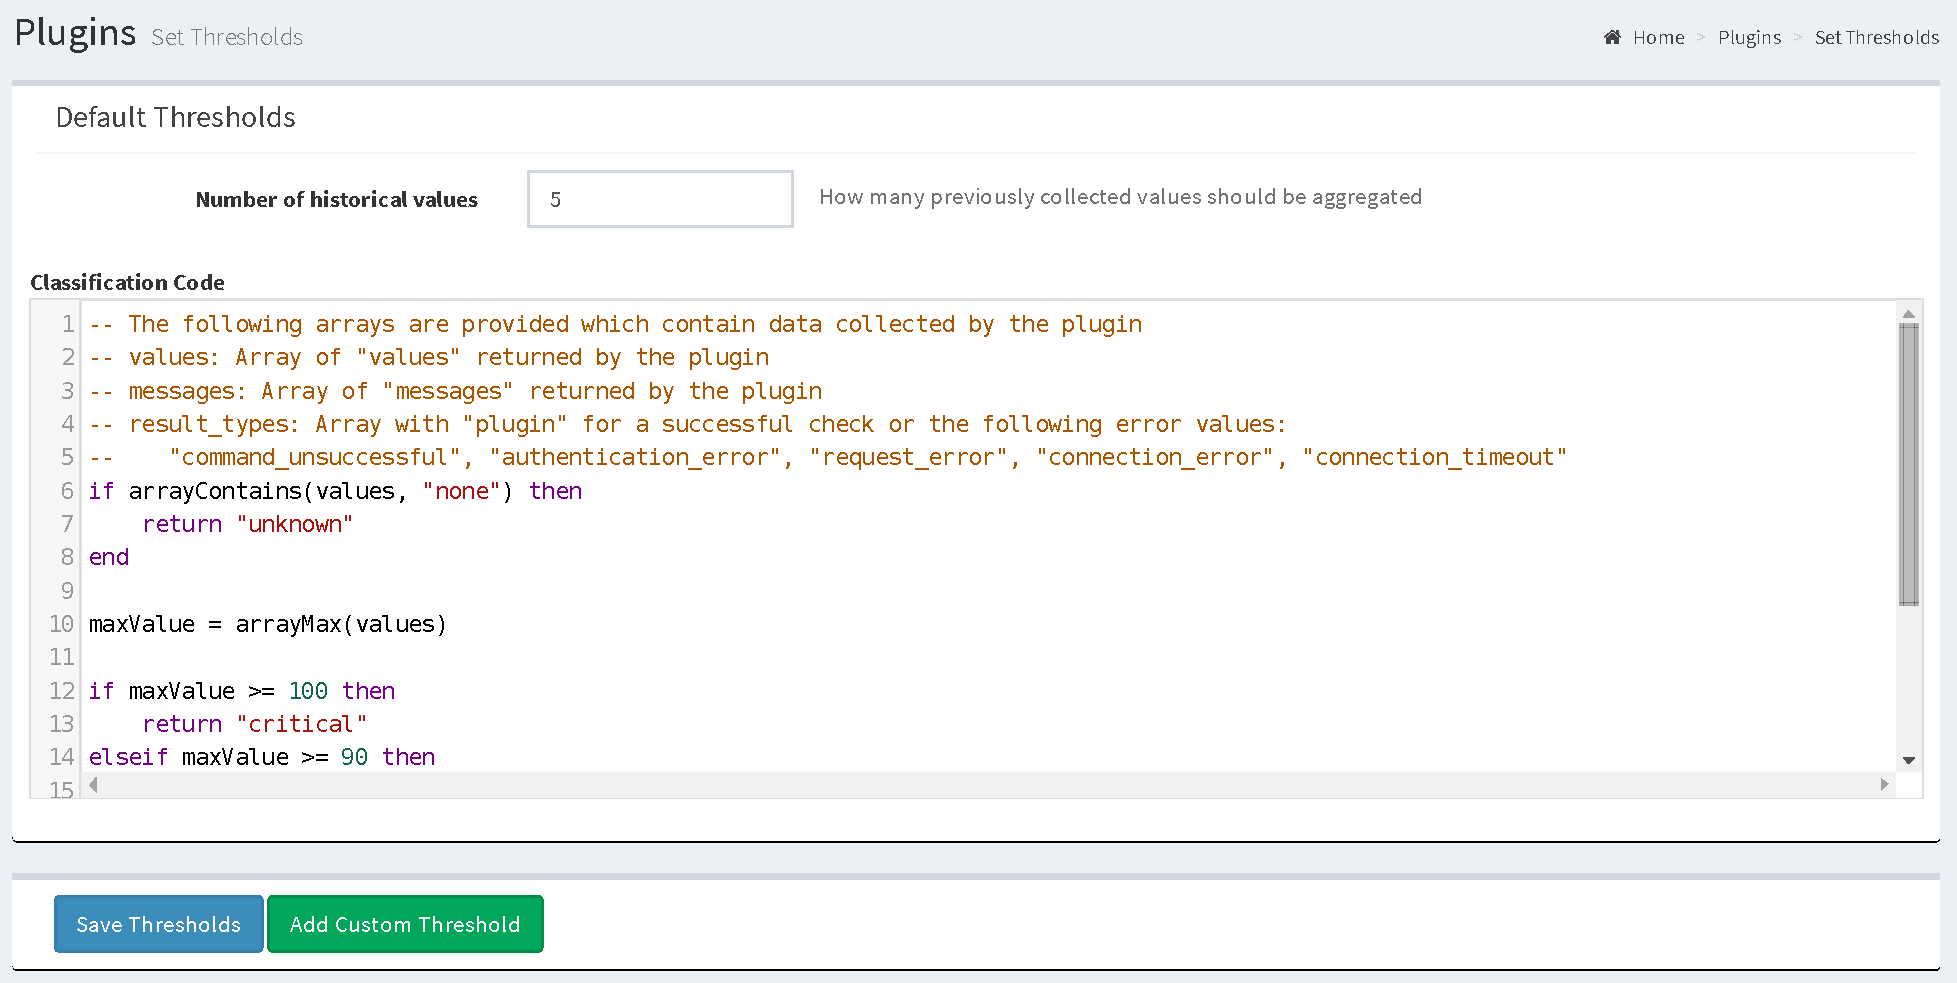
\includegraphics[scale=0.45]{assets/screenshots/set-thresholds.pdf}
\end{figure}

\paragraph*{Schedules}
	As described in Section \ref{methodology-schedules}, a schedule is used to
	define when to execute one or more checks.  The interface for this includes the
	usual form fields for a name for and description of the schedule as well as a
	checkbox list of available checks to execute.  This page also has additional
	functionality to configure the time intervals at which the schedule is run. This
	can be seen in Figure \ref{schedule-intervals}.  Each interval has fields to
	specify the start time for the schedule as well as a text box and drop down menu
	to enter the interval period.  The green ``Add Interval'' button will add another
	row to this list allowing more intervals to be added and the red ``X'' button will
	remove the row it's in from the table.  This is all handled purely in frontend
	JavaScript.

\begin{figure}[H]
	\caption{Form for managing the intervals for a schedule}
	\label{schedule-intervals}
	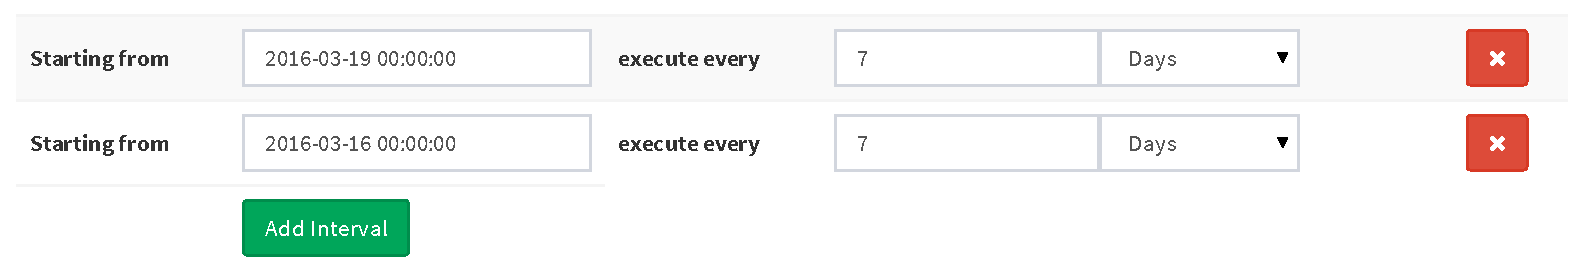
\includegraphics[scale=0.54]{assets/screenshots/schedule-intervals.pdf}
\end{figure}


	In order to display confirmation messages to users,
	Bootbox.js\cite{bootbox} is used which provides a convenient
	abstraction around Bootstrap's build in modal functionality.  This allows
	confirmation messages to be displayed to users without any manual HTML markup
	and responses to be collected straight into JavaScript.  An example of a
	confirmation message can be seen in Figure \ref{bootbox-delete}.

\begin{figure}[H]
	\centering
	\caption{The confirmation message displayed when deleting a plugin}
	\label{bootbox-delete}
	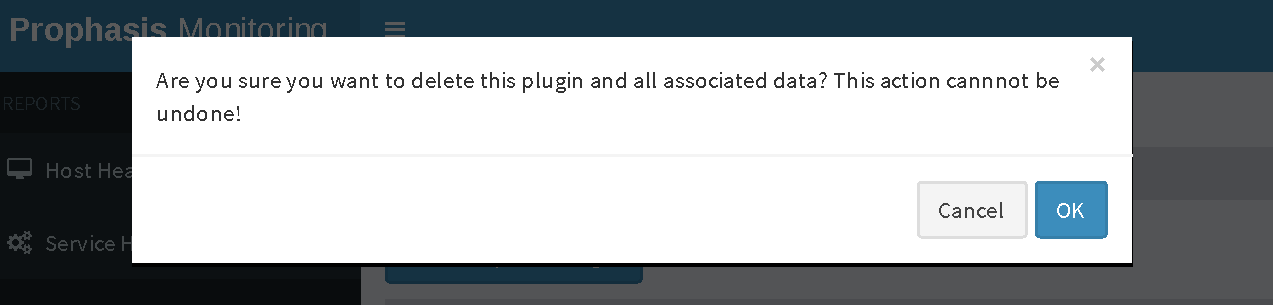
\includegraphics[scale=0.6]{assets/screenshots/bootbox-delete.pdf}
\end{figure}

\paragraph*{Services}
	As described in Section \ref{methodology-services}, services are comprised of
	one or more dependencies or redundancy groups.  Redundancy groups in turn are
	comprised of one or more hosts or host groups.  Building a user interface to
	represent this was particularly challenging as data needed to be represented
	clearly and be intuitive to edit.  The finished interface can be seen in
	Figure \ref{edit-service}.

\begin{figure}[H]
	\centering
	\caption{The user interface for editing services}
	\label{edit-service}
	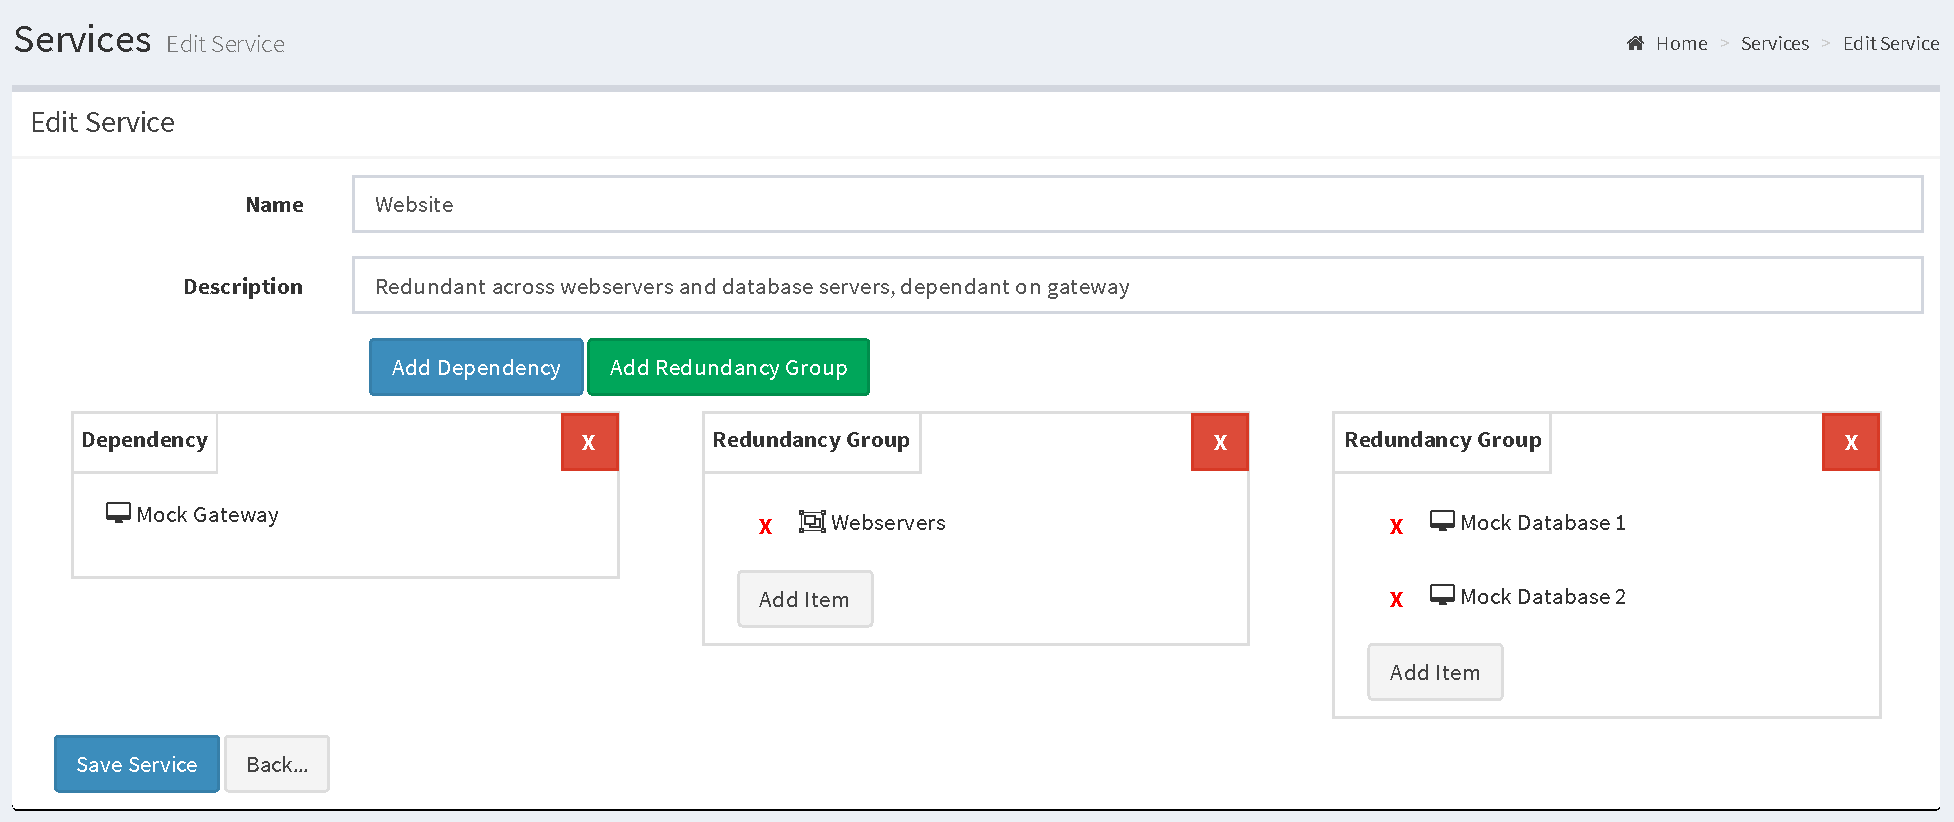
\includegraphics[scale=0.44]{assets/screenshots/edit-service.pdf}
\end{figure}


	In this interface, dependencies and redundancy groups are represented as boxes
	each containing the host(s) and host group(s) that are a member of that
	dependency or redundancy group.  Individual hosts can be added to redundancy
	groups by clicking the ``Add Item'' button or removed by clicking the red ``X''
	next to it.  Entire dependencies can be removed by clicking the red ``X'' in the
	top right of the box.  To select hosts or host groups to create a dependency
	or to add to a redundancy group, a Bootstrap modal dialog is displayed as
	shown in Figure \ref{edit-service-modal}.  On this form, HTML5 data attributes
	are used to attach data such as IDs to the actual DOM elements that represent
	the structure of the service.  When the form is saved, JavaScript is used to
	serialise this structure for processing.  This massively simplifies the code
	as adding and removing dependencies, redundancy groups, hosts.etc can be
	handled entirely in the DOM without having to also maintain a JavaScript data
	structure at the same time.

\begin{figure}[H]
	\centering
	\caption{The modal dialog for selecting hosts and host groups}
	\label{edit-service-modal}
	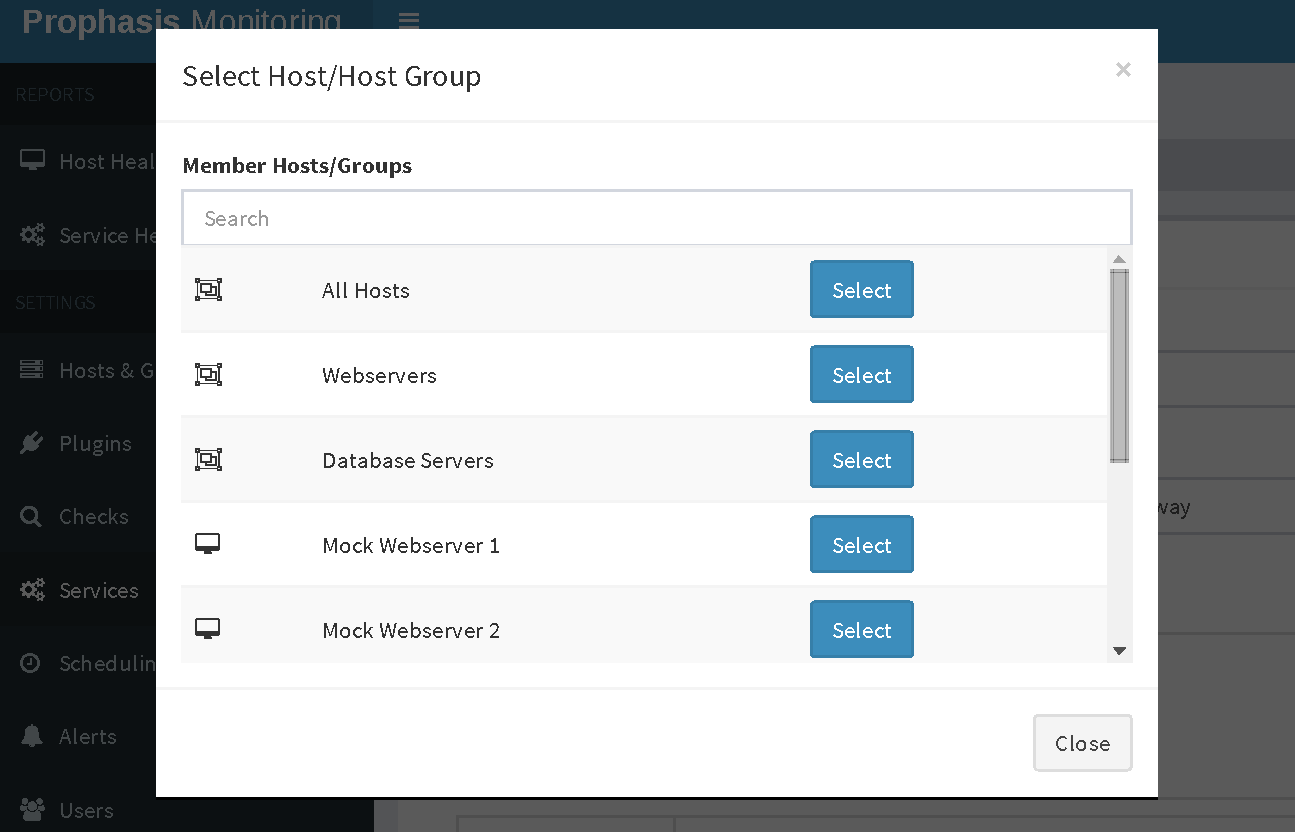
\includegraphics[scale=0.44]{assets/screenshots/edit-service-modal.pdf}
\end{figure}

\subsection{Reporting}

	In addition to being used to configure the system, the web interface is also
	used to visualise the collected data.  There are currently two reports, one
	to show the health of all hosts in the system and another to show the health
	of all services.  There is scope to add more reports to give different views
	of the data.
\subsubsection{Host Health}

	Figure \ref{host-health-index} shows the host health report for
	a selection of machines.  This report lists all the machines in the system
	as well as displaying their health in both a textual and colour representation.
	The results here are sorted in order from least to most healthy.  This ensures
	that even in a network with a large number of systems, unhealthy hosts will not
	go unnoticed due to being buried deep inside a list, especially on the small
	screens of mobile devices.

\begin{figure}[H]
	\centering
	\caption{The index page for the Host Health report}
	\label{host-health-index}
	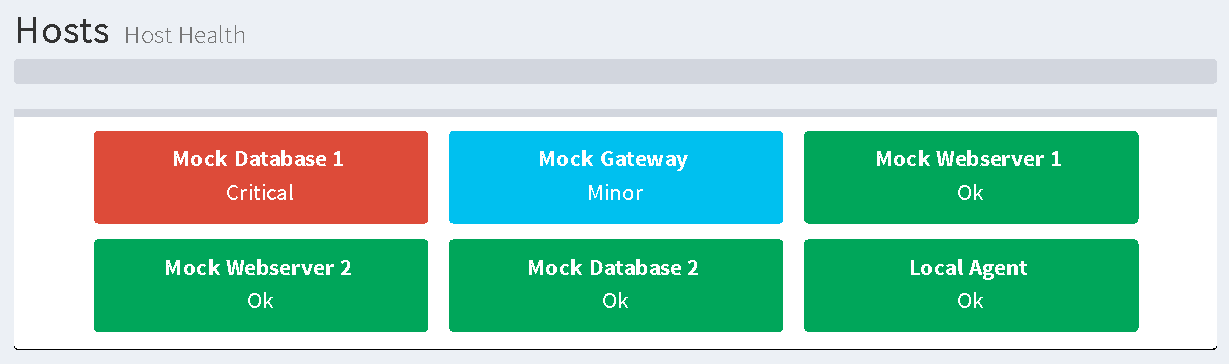
\includegraphics[scale=0.7]{assets/screenshots/host-health-index.pdf}
\end{figure}


	Clicking on any of these hosts will open a page displaying more detailed
	breakdowns of the data stored for that host.  This is where the time series
	data can be visualised.  Figure \ref{host-information} shows a sample
	output of time series data collected from a running server.  This shows both
	the status of the Linux MD RAID devices as well as a graph of CPU load
	showing a large spike due to a RAID consistency check that occurred on the
	machine.  At the top of this report are a pair of inputs allowing the time
	period that the data represents to be specified.

\begin{figure}[H]
	\centering
	\caption{The host information page showing time series data for a single host}
	\label{host-information}
	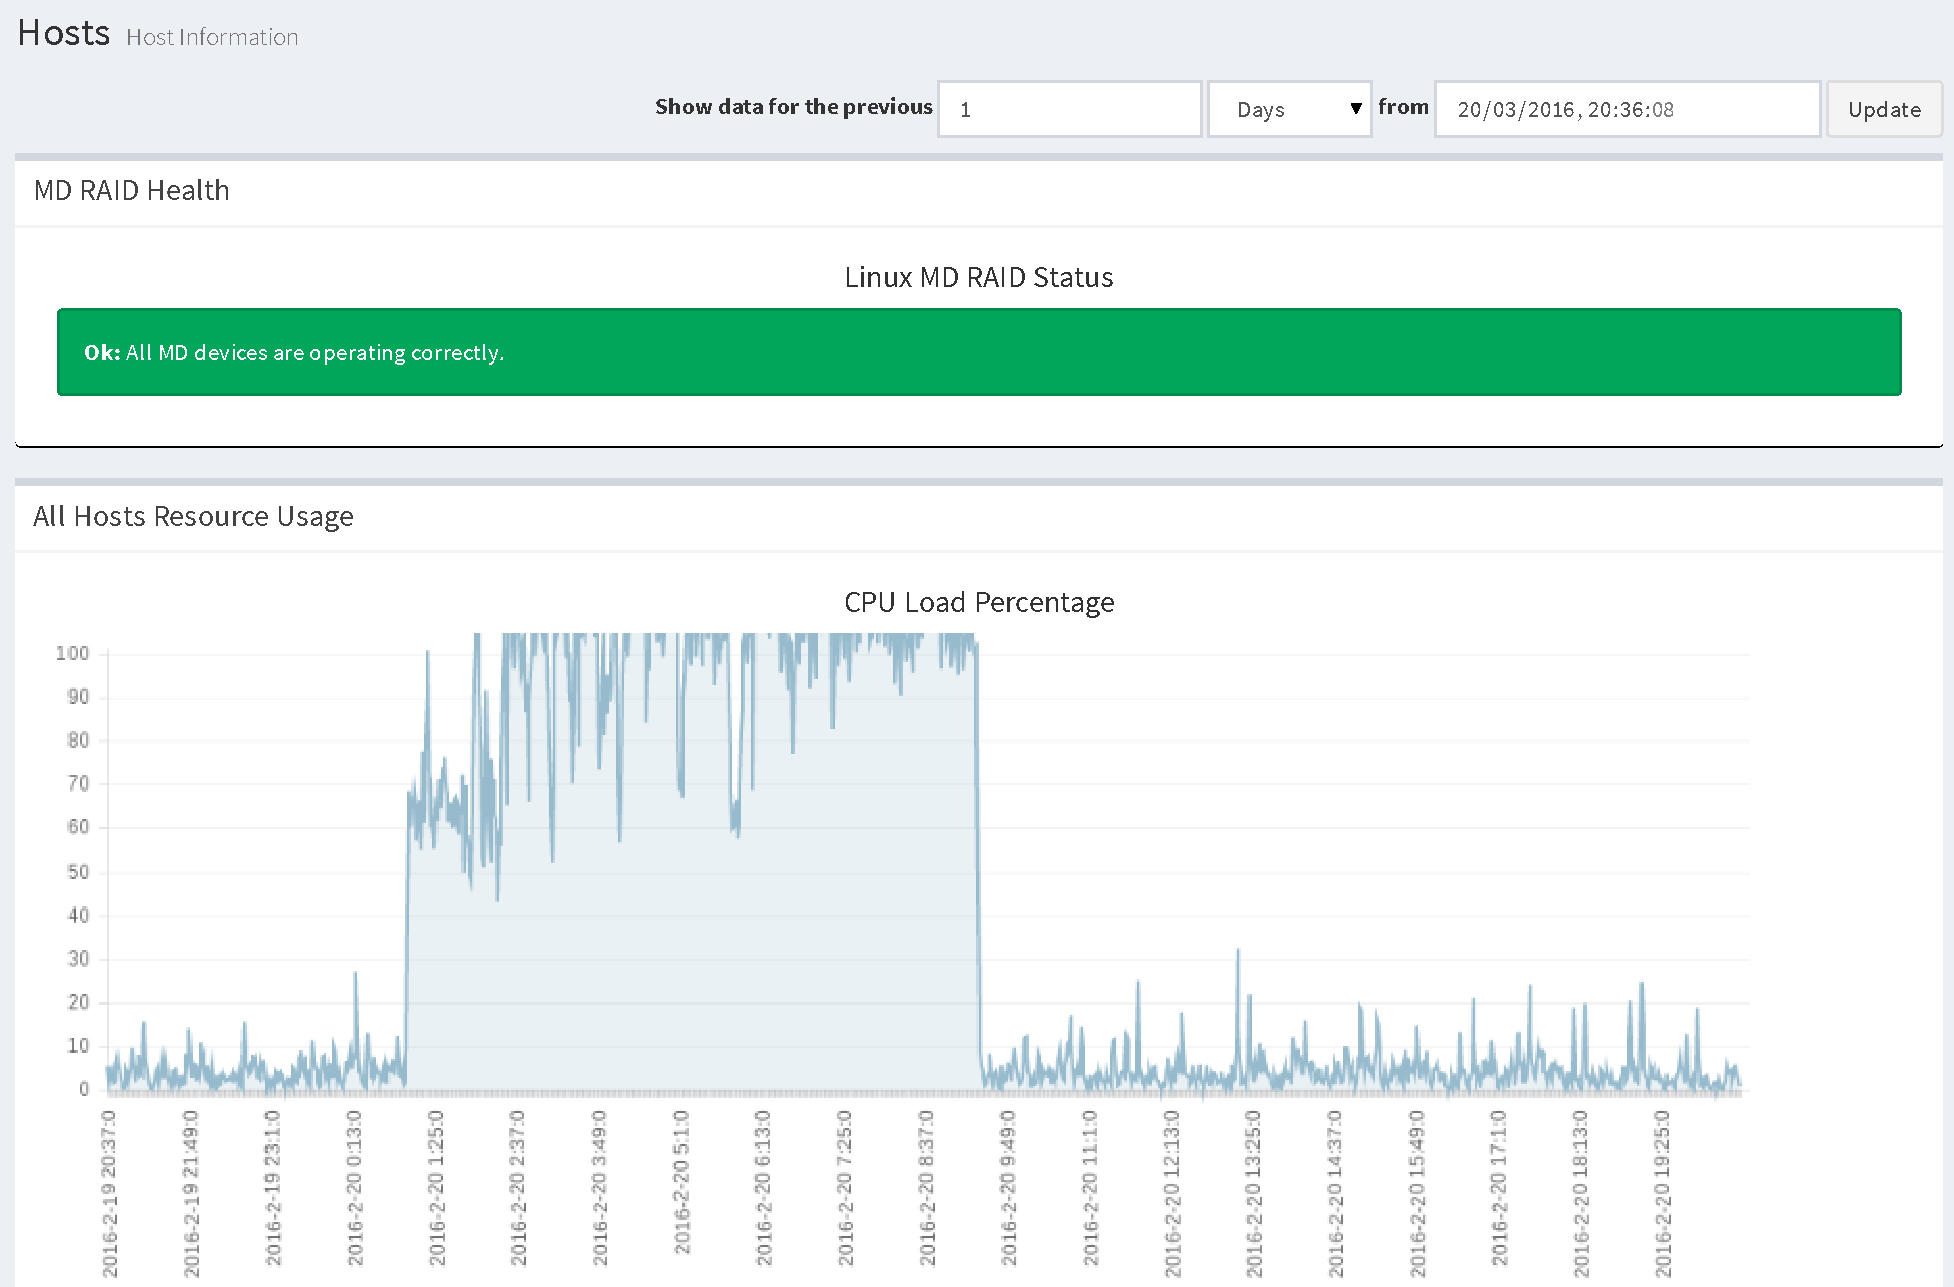
\includegraphics[scale=0.43]{assets/screenshots/host-information.pdf}
\end{figure}

\subsubsection{Service Health}

	In order to give a view of the overall health of the services running on a
	system or to show the impact that a fault with a host has on the overall
	functionality of a system, a report is available to list the health of all
	services.  This is shown in Figure \ref{service-health-index}. Like the
	Host Health report, the services are ordered to show the services with the most
	serious condition first.  As can be seen, services have an additional health
	status of ``Degraded'' which means that while a service is operating normally,
	one of its redundant components is experiencing an issue.

\begin{figure}[H]
	\centering
	\caption{Page showing the overall health of all services in the system}
	\label{service-health-index}
	
\includegraphics[scale=0.6]{assets/screenshots/service-health-index.pdf}
\end{figure}


	Clicking on each of these services will load a view that shows the status of
	all hosts in the service as well as how they are structured in terms of
	dependencies and redundancy groups.  This is shown in Figure
	\ref{service-information}.  Clicking on each of the hosts on this page loads
	the host information view as shown above.  This view clearly shows the reason
	for a service's health status and allows issues affecting a service to be
	clearly seen.

\begin{figure}[H]
	\centering
	\caption{Page showing the overall health of all services in the system}
	\label{service-information}
	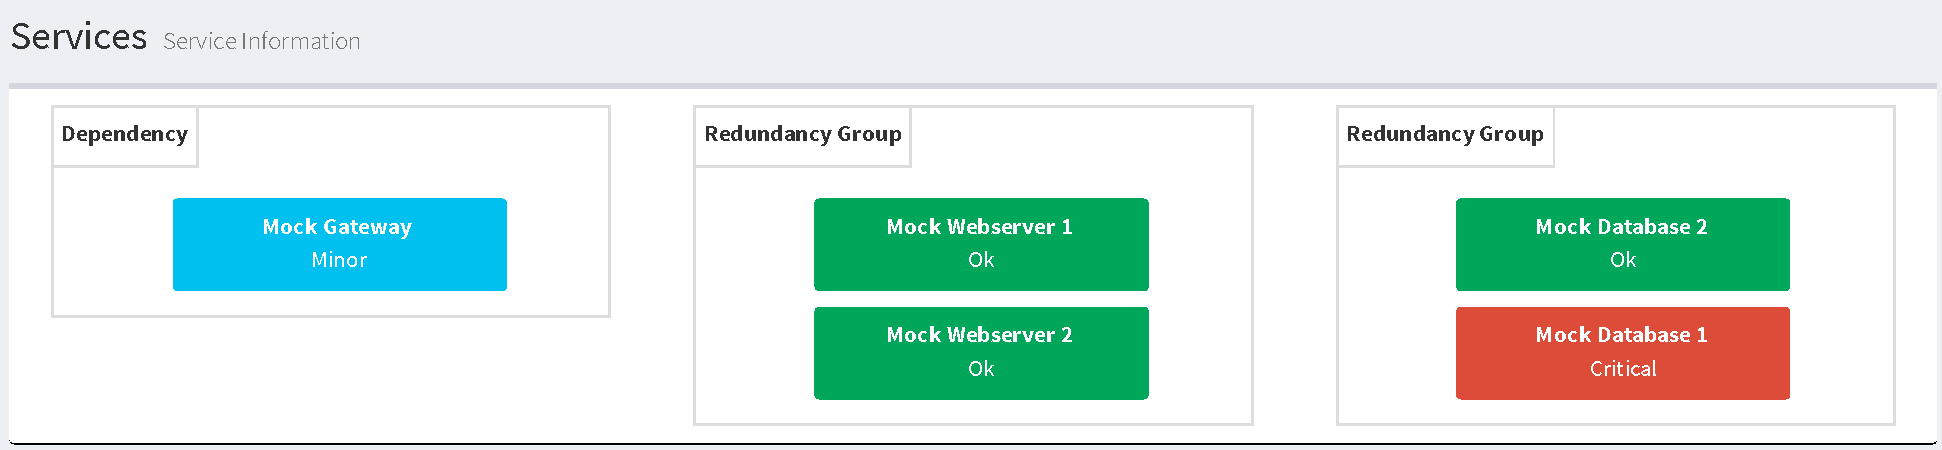
\includegraphics[scale=0.44]{assets/screenshots/service-information.pdf}
\end{figure}

\section{Responsive Design}
	It is important that Prophasis works equally as well on both mobile and desktop
	devices with no loss of functionality on either.  To enable this, a responsive design
	was chosen. This will automatically scale and rearrange the user interface
	based on the screen size.  When being viewed on a small screen, certain items
	that are normally displayed side by side will be stacked as shown with the
	host health screen shown in Figure \ref{responsive-host-health}. The navigation
	bar is also automatically collapsed to save screen space. It can be expanded
	by pressing the menu button (three horizontal lines) in the top left hand
	corner of any page.  This operation of the menu can be seen in Figure 
	\ref{responsive-nav-bar-expanded}.  Forms are also adapted so that they are
	stacked vertically as seen with the alert creation form shown in Figure
	\ref{responsive-alert-form}.
	
\begin{figure}
    \centering
    \begin{subfigure}[b]{0.45\textwidth}
        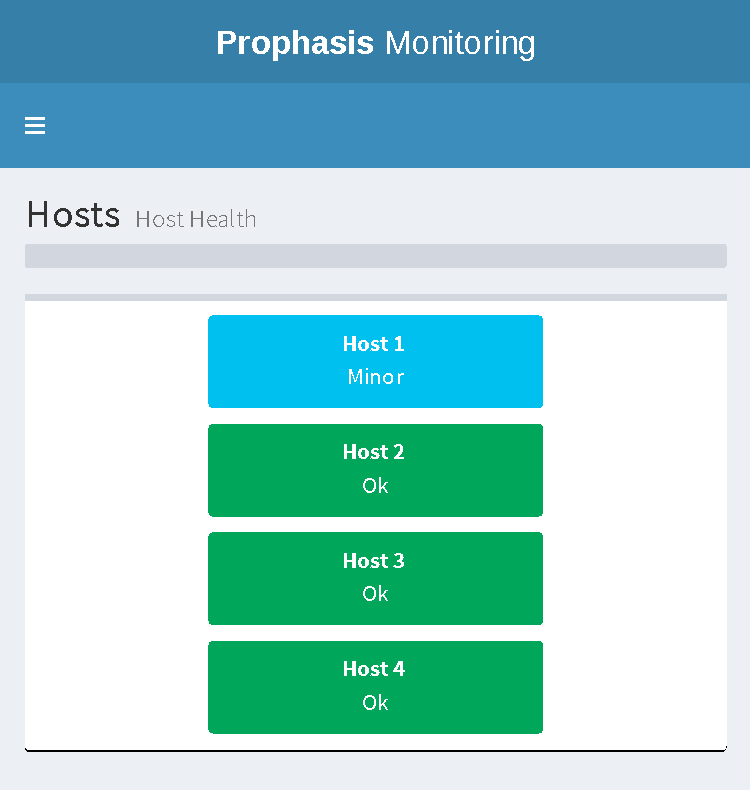
\includegraphics[width=\textwidth]{assets/screenshots/responsive-host-health.pdf}
        \caption{Host Health}
        \label{responsive-host-health}
    \end{subfigure}
    \begin{subfigure}[b]{0.45\textwidth}
        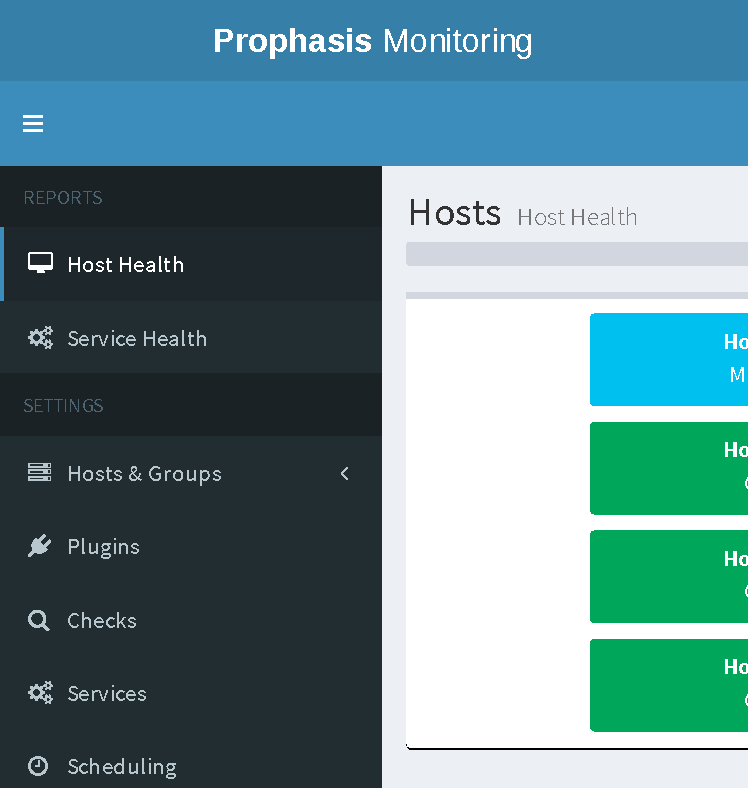
\includegraphics[width=\textwidth]{assets/screenshots/responsive-nav-bar-expanded.pdf}
        \caption{Expanded Navigation Bar}
        \label{responsive-nav-bar-expanded}
    \end{subfigure}

    \begin{subfigure}[b]{0.5\textwidth}
        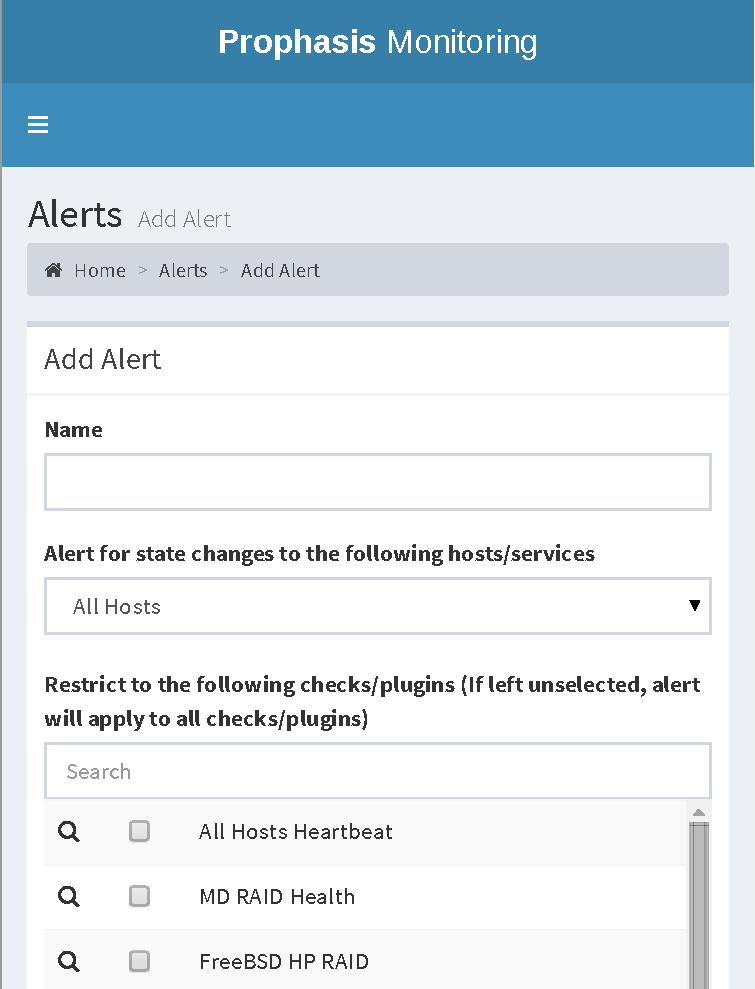
\includegraphics[width=\textwidth]{assets/screenshots/responsive-alert-form.pdf}
        \caption{Alert Creation Form}
        \label{responsive-alert-form}
    \end{subfigure}
    \caption{Parts of the Web Interface being Viewed on a Small Screen}\label{fig:animals}
\end{figure}


\chapter{Testing}
	This chapter explains how Prophasis was tested to ensure both correct operation
	and to evaluate it's general performance.  It first starts off by explaining
	the automated unit testing that was set up on certain, complex functionality
	within the system.  It then explains the ``mock agent'' that was used during
	development to allow easy simulation of a a network containing many different
	hosts.  Finally it goes on to explain the use of Prophasis in real world 
	environments including The Tardis Project within The University of Edinburgh
	as well as in an external company, Lynchpin Analytics Limited.

\section{Unit Testing}

	Unit tests were used to test the more complex functionality of the system such
	as getting all member hosts in a host group or determining the overall health
	of a host or service.  These algorithms are somewhat complex so having unit
	tests was useful to both verify the functionality during development as well
	as to ensure this functionality is not broken by changes to other parts of the
	system.  The Python \texttt{unittest} library was used as it is included as part of
	a standard Python install and is well documented.


	Each test case was implemented as a single class with each different test in a
	separate function within this.  Each \texttt{TestCase} has a \texttt{setUp()}
	method which is called before each test in the class is executed.  The
	\texttt{setUp()} method will drop all database tables, recreate the database
	structure from the models file and will then insert sample data for use in the
	tests.  This ensures that every test starts on a clean database.


	In order to prevent tests from affecting the main database or requiring a new
	database to be set up, SQLite is used.  A temporary, in memory database is
	created when the tests are executed which is then destroyed when the tests are
	completed.  When a test is started it sets an OS environment variable called
	\texttt{UNDER\_TEST}.  If this is set the models module will set the database
	connection string to \texttt{"sqlite://"} instead of the one stored in the config
	file. The SQLAlchemy ORM completely transparently handles the differences
	between PostgreSQL and SQLite therefore requiring no changes to the database
	code for use during testing.
	
	For each function, the input space was divided into inputs that are to be
	expected by the code and tests are used to ensure that the correct output is
	given.  Inputs are also provided that are invalid to ensure that the
	appropriate exceptions are raised.  Inputs are built with the logic under
	test in mind to ensure that behaviour is correct even in edge cases.  For
	example, the test that retrieves a list of hosts inside a host group tests
	the case where group $A$ contains group $B$ and group $B$ contains group $A$.
	If care was not taken, attempting to recursively get a list of hosts from
	either of these groups
	could recurse indefinitely.  Having a test for this case ensures that this does
	not happen.


\section{Mock Agent}

	When developing and testing Prophasis, it was important to be able to simulate a
	network of multiple machines all being monitored and in addition to this it
	was essential to be able to simulate faults with these machines. While it would
	have been possible to run multiple agents and then use plugins to return data
	and to simulate faults this would have been impractical to set up, run and maintain.


	As a solution to this, a mock agent was developed.  This is a simple application
	that implements enough of the agent's functionality to allow the core to
	communicate with it as though it is a regular agent.  It does not use plugins
	and instead reads the data to respond with from a JSON file stored on disk. The
	agent's \texttt{ping} method is implemented as normal, the
	\texttt{check\_plugin\_version} method always responds saying that an update for
	the plugin is not required (this means that the \texttt{update\_plugin} method does
	not need to be implemented).  The \texttt{get\_plugin\_data} method is then
	used to read the JSON file and respond with the appropriate data. Figure
	\ref{mock-agent-data} shows an example of the JSON file used by the agent.

\begin{figure}[H]
	\caption{An example of the JSON file read by the mock agent}
	\label{mock-agent-data}
	\lstinputlisting[basicstyle=\footnotesize\ttfamily,frame=single]{assets/mock-agent-data.json}
\end{figure}


	In order to keep the mock agent simple, it listens on a single port (4048, the
	same as the regular agent) and binds to the system's loopback address 
	(typically \texttt{127.0.0.1}).  Multiple hostnames should then be configured
	to point to the loopback address either through the system's hosts file or on
	the DNS server itself.  For each of these hostnames, a host should be added
	within Prophasis.  The HTTP \texttt{host} request header field is used as the
	key to look up the data to return from the JSON file. This header contains the
	hostname that the core is connecting to allowing, for example, requests for
	data from \texttt{host1} to be differentiated from requests for data from 
	\texttt{host2}.


	The JSON file is read every time a request reaches the mock agent.  This means
	that the test data can be changed on the fly while the mock agent is running by
	simply changing the data in the file and saving it.  For example, to test what
	happens if the CPU load on a machine is too high the value in the JSON file can
	simply be changed to the new CPU load, the next time the CPU
	load plugin is executed on that specific agent, the new CPU load will then be
	sent out.

\section{Use in the Field}

	There is only so much information that can be gained from testing a system such
	% Better word for the environment?
	as Prophasis in a clean environment through the use of the mock agent and unit
	tests.  In order to see how Prophasis performs when deployed in a real world
	environment Prophasis was installed and run in two different real world
	environments.

\subsection{The Tardis Project}
\label{testing-tardis}

	The Tardis Project is a computer system operated and maintained by students at 
	the University of Edinburgh.\cite{tardis}
	It provides services to students including shell accounts, web hosting and mail
	services.  The project currently runs off of 9 physical servers and on these
	operates a large number of virtual machines.


	Prophasis was installed on the Tardis system somewhat early in its development
	so that it could be operated in a running environment 24 hours a day. A virtual
	machine was created to run the core, web interface, an agent and the database,
	the agent was also installed on several different hosts including the shell
	server and the machine that provides network storage to the rest of the system.


	Tardis's primary storage host uses Linux MD RAID to provide redundancy.  For
	this a custom plugin was developed to parse the file at \texttt{/proc/mdstat}
	which provides information about the health of the disks in the system. This
	allowed Prophasis to be able to monitor the health of the Tardis system's
	primary storage.


	The deployment on Tardis was extremely useful as it allowed Prophasis to be
	tested in a real world environment from the very beginning where new features
	could be launched and tested on live servers rapidly.  It also highlighted
	issues that would otherwise be hard to find such as those that only occurred
	infrequently or after the system had been running for a reasonable period of
	time.

\paragraph*{Scheduler Deadlock}
	One issue that was discovered while running on Tardis was where the scheduler
	could, in rare cases completely lock preventing future checks from being
	executed.  This issue was caused where a check could take too long to run
	resulting in the time at which it was next meant to execute being set to a
	time which, by the time the check had completed, was in the past.  The result
	was that the check would never be executed again.  This issue was later solved by
	allowing checks to execute ``late'' up until a defined threshold. If they are
	later than this threshold, the time at which the check is to execute next will
	still be incremented.  This prevents this locking issue from occurring. Since
	this issue occurred very rarely, it was extremely useful to be able to use
	Tardis as the core could be left running 24/7 which allowed this issue to be
	noticed. If Prophasis had only ever been run on a single machine for short
	periods of time during development, it is possible that this issue would never
	have been discovered.  This also highlights the danger of a system such as
	Prophasis deadlocking. In order to ensure that the system cannot deadlock in
	any other way, the scheduler and dispatching algorithms should be checked
	carefully by hand to ensure that there is no situations where a deadlock can
	arise.

\pagebreak
\subsection{Lynchpin Analytics Limited}

	Lynchpin Analytics Limited (``Lynchpin'') is full service analytics
	consultancy.\cite{lynchpin} Lynchpin is a small business yet
	operates a reasonably sized network running entirely on their own hardware.
	This is typical of environment that Prophasis is aimed at and where existing
	tools fall short.  Prophasis was deployed at Lynchpin when it was nearly
	complete in order to evaluate how the finished product works in a heterogeneous
	environment and to highlight any major issues that occur.


	Lynchpin operates a range of vastly different systems which makes it an
	ideal environment to test Prophasis.  Unlike on Tardis where the majority of
	systems run Debian Linux, Lynchpin operates systems running Citrix XenServer (where
	Dom0 is based on CentOS 5), Debian and FreeBSD with a wide variety of different
	types of hardware.  The Prophsis core, database and web interface were
	installed in a Debian Linux Virtual Machine running on one of the XenServer
	hosts.  The agent was then installed on several different systems.  Table
	\ref{table-lypn-hosts} lists the systems on which the Prophasis agent was
	installed.  This allowed me to test Prophasis on a selection of different
	operating system families (Linux, BSD and Windows) and storage configurations
	(Linux MD RAID, Dell Hardware RAID and ZFS on top of an HP SmartArray
	controller).

\begin{table}[H]
	\centering
	\caption{Systems on which Prophasis was installed}
	\label{table-lypn-hosts}
    \begin{tabular}{|l|l|l|}
    \hline
    \textbf{Type} & \textbf{Operating System} & \textbf{Storage} \\ \hline
    Virtual Machine & Debian 8 (Jessie) & Single Virtual Disk Image \\
    Virtual Machine & Windows Server 2012 R2 & Single Virtual Disk Image \\
    HP ProLiant DL180 g6 & FreeBSD 10.2 & ZFS, HP SmartArray P410 \\
    HP ProLiant DL180 g6 & FreeBSD 10.2 & ZFS, HP SmartArray P410 \\
    Dell CS24-SC & Citrix XenServer 6.5 & Linux MD (Software) RAID \\
    Dell CS24-SC & Citrix XenServer 6.5 & Linux MD (Software) RAID \\
    Dell PowerEdge R630 & Citrix XenServer 6.5 & Dell PERC H330 RAID \\
    Dell PowerEdge R630 & Citrix XenServer 6.5 & Dell PERC H330 RAID \\ \hline
    \end{tabular}
\end{table}


	During the time in which Prophasis was installed, one of the XenServer hosts
	experienced a prolonged period of very high CPU load.  Prophasis
	correctly detected this and sent out the appropriate alerts.  It was then 
	possible to look at the time series data for the CPU load on the host which
	had experienced the issue. This data the start and end times of the period
	with high load. This information was useful when looking through log files
	to find the cause of the issue which ultimately turned out to be a MD RAID
	consistency check.


	The deployment was extremely successful with Prophasis reliably monitoring all
	systems.  Performing this deployment on Lynchpin's systems was extremely
	valuable and both demonstrated that Prophasis works well in such a deployment
	and highlighted some improvements that could be made.

\paragraph*{Stability}
	The deployment of Prophasis at Lynchpin has demonstrated the stability of
	Prophasis running in a live environment.  The entire system operated
	successfully for more than a month without requiring any component of the
	system to be rebooted.  Over this time a large amount of historical data has
	been collected and stored within the Prophasis database without causing any
	sort of major performance degradation, this shows that the system will not slow
	down over time due to the database filling up.  There was also no incidents of
	the scheduler locking as described in Section \ref{testing-tardis} which,
	while it doesn't prove the absence of issues of this type, shows that the
	scheduler is stable enough for production use.

\paragraph*{Documentation}
	Deploying Prophasis on several different systems at Lynchpin gave a valuable
	opportunity to document the install process on several different platforms.
	This allowed installation instructions to be written for Debian Linux,
	Citrix XenServer, FreeBSD and Windows.  This also gave insight into subtle
	differences in the availability of different dependencies on different
	platforms such as the lack of Python 3 in the XenServer (CentOS 5)
	repositories, requiring it to be built from source.

\paragraph*{Plugin Development}
	The large number of different storage configurations on which Prophasis was
	deployed provided a valuable opportunity to develop plugins for the different
	storage configurations.  A plugin was developed to read the health of the
	drives running on an HP SmartArray P410 RAID controller under FreeBSD through
	the use of \texttt{camcontrol}.\cite{smartarray-bsd}  Another plugin was written to check the
	health of a ZFS zpool which executes \texttt{zpool status} and parses the
	output.  In order to check the health of the disks running behind the Dell PERC
	H330 RAID controller, a plugin was developed which read SMART data by calling
	\texttt{smartctl} with \texttt{-d megaraid,nn} to access the disks behind the
	Dell PERC (a rebranded LSI MegaRAID) RAID controller.\cite{smartctl-megaraid}

\paragraph*{Plugin Execution Timeouts}
	While testing the deployment at Lynchpin, an issue was discovered with the
	plugin that was checking the zpool status on the machines using ZFS. One of the
	hosts developed an issue resulting in the \texttt{zpool status} command simply
	hanging.  Prophasis had no timeout for this so once this plugin had been
	executed, any future plugins would be stuck in the dispatch queue in the core
	and would never be executed (due to the one simultaneous check per host
	policy).  The solution for this was to implement timeouts on the agent so that
	if a plugin takes longer than a predetermined time limit to execute, the
	execution will be terminated and an error would be logged.  This prevented
	the dispatch queue from being blocked up in the event of a long/infinitely
	running plugin.

\paragraph*{Windows Support}
	The agent was deployed on a virtual machine running Windows Server 2012 R2
	Standard, this provided an opportunity to test the behaviour of the Prophasis
	agent when running under Windows (previously it had only ever been executed on
	UNIX-like operating systems).  It was found that the ``timeout-decorator''
	library being used to allow plugin execution to halted if a plugin was taking
	too long to execute used \texttt{SIGALRM} signals which are not supported by
	Windows. The solution was to swap the ``timeout-decorator'' library out for
	``stopit'' which can use multithreading to implement timeouts instead of UNIX
	signals.  This solution works Windows as well as UNIX-like operating systems.

\paragraph*{Ideas for Future Work}
	Deploying and using Prophasis at Lynchpin provided several ideas for future
	features that could be implemented.  While the system
	was operating, one of the XenServer hosts automatically checked the consistency of
	its RAID arrays.  This resulted in extremely high CPU load which sent out
	alerts warning of this issue despite this being standard operation. Future work
	to solve this could involve allowing data from one plugin to be retrieved when
	classifying data from another plugin. This would mean that the CPU load
	classification logic could be configured to ignore CPU load caused by MD RAID
	checks on any hosts which use Linux MD RAID. It was also determined that it
	would be useful to be able to pass arguments into plugins from the core.  This
	means that, for example, a plugin could be written to check the free space
	available on a disk and the disk to check could be specified through an
	argument to the plugin. This would allow different checks to be created to
	check the free space on different disks.  These features are described in more
	detail in Section \ref{future-work}


	Testing Prophasis by deploying it at Lynchpin was incredibly useful. Lynchpin
	as a company perfectly suits the type of environment that Prophasis is designed
	for. Testing showed that Prophasis works reliably in such an environment.  It also
	provided a valuable opportunity to test on a wide selection of software
	platforms and hardware configurations to ensure software support.  Deployment
	also indicated some potential issues which have now been resolved as well as
	inspiring ideas for future features and enhancements.

\chapter{Evaluation}
	This chapter starts off by evaluating Prophasis against the same points which
	existing tools were evaluated against in Section
	\ref{analysis-of-existing-tools} to demonstrate the improvements made. It then
	goes on to describe future work that could be implemented in order to further
	enhance the functionality of the system.

	Prophasis is now a complete system that is sufficiently developed to be able to
	be deployed on a network.  It has been tested both in a synthetic environment
	and on multiple real world networks.  The complete system improves on
	the points at which current systems tend to fall short as described in Section
	\ref{analysis-of-existing-tools}. These improvements are described below.

\paragraph*{Time series monitoring and real time alerting}
	Prophasis has support for both time series monitoring and real time alerting
	built in.  Time series data is tightly integrated into the system rather than
	being bolted on later meaning that historical data can be used to make
	decisions such as deciding the overall health of a host.  This is a clear improvement
	on existing tools where they traditionally only support time series monitoring
	or real time alerting.

\paragraph*{Support for Custom Metrics}
	Like all other tools, Prophasis supports monitoring custom metrics using custom
	code.  Prophasis however has a much more rigid structure for plugins which
	helps to ensure consistency and reliability of plugins.

\paragraph*{Classification Threshold Definitions}
	This is an area where Prophasis clearly improves on existing systems.  Other
	systems rely on the plugin code that is executed on the remote host to
	determine and return the overall classification. As a result, classification
	logic is stored in various locations spread out all over the network which makes
	management difficult.  In
	Prophasis, plugins simply return a raw
	value that represents the collected data. Classification is then done by user
	provided Lua code on the monitoring server itself.  This means that
	classification code is all stored in one place and can be edited directly from
	the web interface.  Classification code also has access to historical data so
	it can make better decisions than it could if it only knew the current state of
	a host.  Using short blocks of Lua code provides total flexibility to allow any
	sort of logic to be used to classify the data instead of simply having
	rigid thresholds defined through a form in the web interface.

\paragraph*{Code/Configuration Delivery to Nodes} %TODO Config?
	This is another area that Prophasis has improved on.  Current systems rely on code for
	custom plugins to be stored on the machines being monitored but do not provide
	functionality to handle this.  This requires a separate tool such as Puppet or
	Ansible to manage this. Tools such as these may not be in
	place on smaller networks where each machine has a very distinct role which
	reduces the need for centralised configuration management.  In contrast,
	Prophasis stores a central repository of all plugins on the monitoring server
	and distributes these to remote agents automatically.  This means that plugins
	only need to be updated in one place by uploading the plugin archive through
	the web interface. Prophasis transparently handles the rest.

\paragraph*{How the user configures the system}
	Current tools store all of their configuration settings in files stored on
	disk. These require a deep understanding of the system to configure and
	maintain. In Prophasis, configuration files only store the minimum amount of
	information required for the system to be able to start such as database
	connection settings.  The majority of configuration relating to checks, alerts,
	schedules.etc is stored in the database and managed through clearly laid out
	forms in the web interface.  The web interface contains help text and
	explanations of various terms as well as validating user provided input to
	prevent invalid configuration being saved.

\paragraph*{How Dependencies are Handled}
	Unlike many current tools which only support simple \texttt{AND} dependencies
	which require all hosts to be operational,
	Prophasis has a flexible system for handling dependencies. A service can be
	configured as being dependent on all specified hosts being accessible (an
	\texttt{AND} dependency) or can be configured for redundant systems where the
	availability of a service requires at least one host from a set of hosts to be
	accessible (an \texttt{OR} dependency).  Various different combinations of
	\texttt{AND} and \texttt{OR} dependencies are possible.  This allows alerts to
	be fine tuned preventing unnecessary alerts resulting from minor faults in a
	highly redundant environment.


\section{Future Work}
\label{future-work}

	While Prophasis is now a complete system which could be (and has been) used in
	production environments in its current form, there are additional
	enhancements and functionality which could be added to the system to improve
	it even further.
	
\paragraph*{Distributed Monitoring}
	The Prophasis core currently runs on a single host and monitors all other
	hosts in the network.  This is sufficient for most small to medium sized
	networks (the ones Prophasis targets) but provides no redundancy in terms of
	the monitoring system.  If the Prophasis host were to fail then no alerts would
	be sent out. This could be made worse if Prophasis shared a physical machine
	with more critical services and this machine was to fail as critical services
	would become unavailable but since Prophasis has also failed, notifications
	would be sent out.  A solution to this would be to build in support for multiple
	cores to be operating simultaneously where each monitors it's own set of nodes.
	This could be implemented through the use of database replication to keep the
	database in sync across all monitoring nodes.  One node would then be
	designated the ``master'' and would handle the web interface, all other nodes can
	only insert the results of checks into the database which would reduce the
	complexity involved.  This could be enhanced with functionality to
	automatically ``repair'' the monitoring system in the event of a monitoring node
	failure by assigning the hosts that the failed node was responsible for
	monitoring amongst the remaining monitoring nodes.

\paragraph*{Server-side Plugins}
	Currently, plugins are executed exclusively on the host they are checking. This
	additional feature would allow plugins to be marked as ``server-side'' meaning
	that they are executed by the core and run on the monitoring node instead of
	the agent.   Plugins of this type could check external availability of services
	running on a host such as ensuring that a web server is listening externally
	and that no firewalls are blocking traffic.  Server-side plugins could also be
	used to check devices that cannot run the Agent directly such as routers and
	switches.  In this case a server-side plugin could be written to communicate
	with these devices over SNMP.

\paragraph*{Access another plugin's data in classification logic}
	Currently, the classification logic for a plugin can only obtain the previous
	$n$ values that were collected for that plugin itself.  This feature would
	allow one plugin to read data from another plugin for use when it is deciding
	how to classify the data.  For example, a CPU load monitoring plugin may want
	to pull in a list of running processes so that it does not alert about high CPU
	load when a known ``safe'' process is using a large amount of CPU. Another
	example of this could be for a plugin that monitors the temperatures in a
	system where it may want to have different temperature thresholds based on the
	current CPU load of the system.

\paragraph*{Passing arguments into plugins}
	This feature would allow plugins to accept arguments when they are executed.
	These arguments would be specified at the check level so that multiple checks
	can be configured to execute the same plugin but with different arguments. An
	example of this would be a plugin to check if a certain process is running on
	a system.  It would be impractical to have a different plugin to check each
	process so a general one could be developed where the name of the process it
	is checking for can be passed in as an argument.  It would then be possible to
	have a check to check if the web server is running by passing ``httpd'' in as the
	argument and another check that uses the same plugin to check that the database
	server is running where ``postgres'' is passed in as the argument.

\paragraph*{External API}
	An API could be developed to allow data collected by Prophasis to be accessed.
	This would allow external tools to be integrated with for various different
	tools.  This could allow deeper analysis and better use of the collected data
	such as automatically provisioning additional servers on a cloud platform in
	the event of current hosts becoming overloaded.  This API could also be used
	to manage the configuration of the system such as adding new hosts
	automatically which would be particularly important in cloud environments where
	hosts are created and destroyed on a regular basis, often automatically.

\paragraph*{Documentation}
	Currently there is very little in the way of documentation explaining how to
	configure and operate the system as well as information about developing
	plugins.  A large amount of future work would be to write comprehensive
	documentation about the system instead of relying on using the source code as a
	reference.

\paragraph*{Nested Services}
	Currently services can be defined as a set of \texttt{AND} and \texttt{OR}
	dependencies across hosts and host groups.  This functionality could be
 	enhanced by allowing these dependencies to factor in the health of other
 	services thereby reducing duplication of dependency structure.  For example,
 	a website may be redundant across multiple web server hosts and also be
 	dependant on the availability of the storage service.

\paragraph*{Daemon Generation during Setup}
	In a deployment the agent, core and web interface should be run as a daemon.
	Currently when the system is installed the daemon needs to be created manually,
	the way this is done varies between operating systems. Future work could
	involve enhancing the setup scripts that are included with the agent, core and
	web interface so that they detect the operating system they are running under
	and perform the appropriate tasks to install the component correctly as a
	daemon.  Doing this would greatly ease the setup process.
	
\paragraph*{Testing}
	Prophasis has already been tested with both unit tests as well as through
	deployment in multiple real world environments.  It would however be valuable
	to extend the unit test suite to provide higher code coverage.  It would also
	be useful to formally analyse the algorithms in the scheduler and dispatcher
	to ensure that they perform reliably without the risk of deadlocks occurring.

%TODO - Links in Bibliography instead of footnotes

\chapter{Conclusion}
	From personal experience in an SME environment and The Tardis Project weaknesses
	were discovered in current IT infrastructure monitoring tools in terms
	of their suitability for the SME sector.  This project examined in depth the
	suitability and limitations of existing tools to develop a complete system to
	suit the specific needs of the SME sector.
	
	
	Research was split into two areas.  Firstly existing tools namely Nagios, Icinga2,
	Munin, collectd and OpenNMS were reviewed.  In the second part the design of a
	tool for use in the SME sector was researched.
	
	
	From the research carried out it was found that existing tools are often
	complex to set
	up and configure and often only provide part of the information required to
	monitor a network meaning that multiple tools are required in order to gain a
	sufficient level of monitoring.
	
	In order to sufficiently monitor a network it is important to have both real
	time alerting to provide notifications about issues along with time series
	monitoring which can be used to both investigate issues post-mortem along with
	being usable to predict future issues before they occur.  Many existing tools
	only provide one of these which means that businesses need to deploy and
	maintain two different pieces of software to monitor their network.  Prophasis
	was developed with support for time series monitoring and real time alerting
	from the very beginning.  This means that only one tool needs to be deployed
	and managed to gain a suitable level of monitoring.
	
	Current tools are generally configured through configuration files stored on
	various different hosts on the network.  This requires both an expert user to
	edit as well as some sort of configuration management tool to ensure that
	configuration is kept consistent across the network.  In contrast, Prophasis
	can be managed from a single, responsive web interface with all configuration
	management being handled internally.
	
	It is important for an IT infrastructure monitoring system to be easily
	expandable for monitoring custom hardware/software.  Most current tools
	rely on custom scripts with no defined structure to be manually set up on
	remote hosts being monitored.  Prophasis, on the other hand, has a clear
	structure for plugins which are stored as self contained ``packages''. Plugin
	packages can simply be uploaded to the monitoring server and assigned to
	specific hosts.  Prophasis handles the rest by distributing the plugin to the
	correct hosts.
	
	%TODO Make into English
	One improvement would be to perform more testing on the finished system. It
	was only used in a production environment for a month during which only minor
	issues arose.  If it were to have been deployed for longer there would be a
	higher likelihood of a more serious problem arising allowing Prophasis's
	behaviour when detecting major faults to be investigated further. It would
	also be beneficial to increase unit testing to have higher code coverage.
	Formal methods could also be used to analyse algorithms in order to ensure
	there is no risk of faults such as deadlocks.


	In conclusion, the project demonstrated that current tools are not best suited
	for use in SME environment and that it was possible to develop a fit for purpose
	solution. Prophasis improves on these issues and provides a complete system that
	is ready for use in a real world environment.  It has been tested in both
	synthetic and real world environments and performed reliably in both.  There is
	a large amount of scope for future expansion and enhancements however, in its
	current form, Prophasis is sufficiently complete for use in a production
	environment.
	
%TODO
%	Future work "such as", "my recommendation"

%TODO Formatting?  Should Prophasis be in itallics throughout?
%TODO Bit in intro about only doing time series or alerting, make this a bit
%	weaker due to OpenNMS.

	\bibliography{bibliography}
	\bibliographystyle{plain}
\end{document}
